% ============================================================
%  chapter02_slides.tex
%  Chapter 2: Derivatives and Gradients
%  Algorithms for Optimization (2nd ed., 2026)
%  Kochenderfer & Wheeler --- MIT Press
%  Reader-friendly edition: complete sentences, symbol glossaries,
%  worked numerical examples, "How to Read This" explanations.
% ============================================================
\documentclass[aspectratio=169,10pt]{beamer}

\usetheme{Madrid}
\usecolortheme{seahorse}

% -- packages ------------------------------------------------------------------
\usepackage{amsmath,amssymb,bm}
\usepackage{graphicx}
\usepackage{booktabs}
\usepackage{listings}
\usepackage{xcolor}
\usepackage{tikz}
\usetikzlibrary{shapes,arrows,positioning,calc}
\usepackage{pgfplots}
\pgfplotsset{compat=1.18}
\usepackage{mathtools}
\usepackage{array}
\usepackage{multirow}

\graphicspath{{figures/}}

% -- listings style ------------------------------------------------------------
\definecolor{codegreen}{rgb}{0.0,0.5,0.0}
\definecolor{codeblue}{rgb}{0.0,0.0,0.7}
\definecolor{codegray}{rgb}{0.5,0.5,0.5}
\definecolor{codepurple}{rgb}{0.5,0.0,0.5}

\lstdefinestyle{pythonstyle}{
  language=Python,
  basicstyle=\ttfamily\scriptsize,
  keywordstyle=\color{codeblue}\bfseries,
  stringstyle=\color{orange},
  commentstyle=\color{codegreen}\itshape,
  numberstyle=\tiny\color{codegray},
  numbers=left,
  stepnumber=1,
  numbersep=5pt,
  frame=single,
  backgroundcolor=\color{gray!7},
  breaklines=true,
  showstringspaces=false,
  tabsize=4,
  captionpos=b,
}
\lstset{style=pythonstyle}

% -- beamer setup --------------------------------------------------------------
\setbeamertemplate{footline}[frame number]
\setbeamertemplate{navigation symbols}{}
\setbeamersize{text margin left=0.5cm, text margin right=0.5cm}

% -- macros --------------------------------------------------------------------
\newcommand{\x}{\mathbf{x}}
\newcommand{\g}{\mathbf{g}}
\newcommand{\G}{\mathbf{G}}
\newcommand{\R}{\mathbb{R}}
\newcommand{\grad}{\nabla}
\newcommand{\T}{^\top}

% -- title ---------------------------------------------------------------------
\title[Ch.2: Derivatives \& Gradients]{%
  Chapter 2: Derivatives and Gradients}
\subtitle{Algorithms for Optimization, 2\textsuperscript{nd} ed.\ (2026)}
\author{Kochenderfer \& Wheeler \\ {\small Slides prepared for lecture}}
\institute{MIT Press}
\date{2026}

% =============================================================================
\begin{document}
% =============================================================================

\begin{frame}
  \titlepage
\end{frame}

\begin{frame}{Chapter Outline}
  \tableofcontents
\end{frame}

% =============================================================================
\section{1. Scalar Derivatives}
% =============================================================================

\begin{frame}[allowframebreaks]{Motivation: Why Do We Need Derivatives?}

  Optimization is the process of finding an input value --- a \emph{design point}
  --- that makes some objective function as small (or as large) as possible.
  To search efficiently, we need a way to answer the question:
  \textbf{``If I change my input slightly, does the function go up or down?''}
  That question is answered by the \emph{derivative}.

  \medskip
  The \textbf{derivative} of a function $f$ at a point $x$ tells us the
  \emph{instantaneous rate of change} of $f$ with respect to $x$.
  Concretely, it is the slope of the straight line that just touches (is
  tangent to) the graph of $f$ at the point $x$.
  When the derivative is positive, $f$ is increasing at $x$; when it is
  negative, $f$ is decreasing; when it is zero, we may be at a local minimum
  or maximum.

  \medskip
  \begin{columns}[T]
    \column{0.58\linewidth}
    In one dimension the derivative is written $f'(x)$ (read ``f prime of x'')
    or equivalently $\dfrac{df}{dx}$ (read ``d-f over d-x'', Leibniz notation).
    In multiple dimensions --- when $f$ takes a vector of inputs --- the
    analogous object is the \textbf{gradient}, written $\nabla f(\x)$
    ($\nabla$ is called \emph{nabla} or \emph{del}).
    Knowing the gradient, a gradient-based optimizer moves the design point
    in the direction that most rapidly decreases $f$ --- this is the
    foundation of virtually every modern optimizer.

    \column{0.38\linewidth}
    \centering
    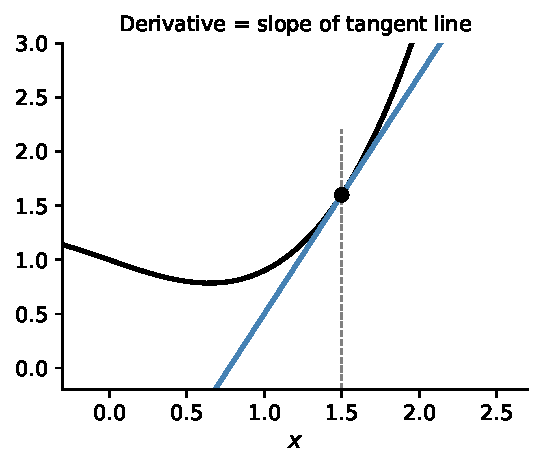
\includegraphics[width=\linewidth]{fig_tangent_line.pdf}\\
    {\scriptsize The derivative equals the slope of the tangent line at
    each point on the curve.}
  \end{columns}

  \medskip
  \begin{alertblock}{Key Takeaway}
    The derivative (in 1-D) and the gradient (in higher dimensions) encode
    the local slope of the objective function.  An optimizer uses this
    information to decide which direction to step next.
  \end{alertblock}
\end{frame}

% ------------------------------------------------------------------------------
\begin{frame}[allowframebreaks]{Scalar Derivative: Formal Definition}

  Intuitively, the derivative is ``how much does $f$ change when I nudge
  $x$ by a tiny amount $h$?'', normalized by the size of that nudge.
  The formal definition takes this idea to the limit as the nudge $h$
  shrinks to zero.

  \begin{block}{Definition of the Derivative}
    The \textbf{derivative} $f'(x)$ of a function $f:\mathbb{R}\to\mathbb{R}$
    at the point $x$ is defined as:
    \[
      f'(x)
        \;=\; \lim_{h\to 0}\frac{f(x+h)-f(x)}{h}
        \;=\; \frac{\Delta f(x)}{\Delta x}
    \]
  \end{block}

  \begin{block}{Notation}
    \begin{itemize}
      \item $f:\mathbb{R}\to\mathbb{R}$ means $f$ takes a single real number
            as input and produces a single real number as output.
      \item $h$ is a small real number representing the size of the
            perturbation (nudge) applied to $x$.
      \item $\lim_{h\to 0}$ (read ``the limit as $h$ approaches zero'') means
            we imagine $h$ becoming arbitrarily small, but never actually
            reaching zero.
      \item $\Delta f(x)$ (``Delta f of x''; $\Delta$ is pronounced
            \emph{Delta}) denotes the change in $f$, i.e., $f(x+h)-f(x)$.
      \item $\Delta x$ (``Delta x'') denotes the change in the input, i.e., $h$.
    \end{itemize}
  \end{block}

  \begin{alertblock}{How to Read This Formula}
    The fraction $\dfrac{f(x+h)-f(x)}{h}$ is the slope of the straight
    line connecting the two points $(x,\,f(x))$ and $(x+h,\,f(x+h))$ on
    the graph.  As $h$ shrinks toward zero, this secant line rotates until
    it touches the graph at exactly one point --- the tangent line.
    Its slope is $f'(x)$.
  \end{alertblock}

  \framebreak

  Three mathematically equivalent ways to write the same limit arise from
  choosing which side of $x$ to nudge toward.

  \begin{block}{Three Equivalent Limit Forms}
    \begin{align*}
      f'(x) &= \lim_{h\to 0}\frac{f(x+h)-f(x)}{h}
               & & \text{(forward: nudge to the right)} \\[6pt]
             &= \lim_{h\to 0}\frac{f(x+h/2)-f(x-h/2)}{h}
               & & \text{(central: symmetric bracket around }x\text{)} \\[6pt]
             &= \lim_{h\to 0}\frac{f(x)-f(x-h)}{h}
               & & \text{(backward: nudge to the left)}
    \end{align*}
  \end{block}

  All three give exactly the same limit --- they are three different ways to
  approach the same tangent slope.  In practice, however, when $h$ is
  kept \emph{small but nonzero} (as in numerical computation), the central
  form turns out to be more accurate.  We will see precisely why when we
  analyze finite differences in Section~3.

  \medskip
  \textbf{Linear approximation interpretation.}
  Because the derivative is the slope of the tangent line, we can
  approximate $f$ near $x$ by that line:
  \[
    f(x + \Delta x) \;\approx\; f(x) + f'(x)\,\Delta x
  \]
  This says: if you move by a small amount $\Delta x$ (``Delta x'',
  the change in $x$), the function value changes by approximately
  $f'(x)\,\Delta x$.  The approximation is accurate when $\Delta x$ is
  small relative to the scale on which the slope changes.

\end{frame}

% ------------------------------------------------------------------------------
\begin{frame}[allowframebreaks]{Symbolic Differentiation}

  The most familiar way to compute a derivative is \emph{symbolic
  differentiation}: applying the rules of calculus (power rule, product
  rule, chain rule, etc.) to the algebraic expression for $f$ and
  producing an exact algebraic expression for $f'$.

  \medskip
  \textbf{Example (analogous to Example 2.1 in the textbook).}
  Consider the function
  \[
    f(x) = x^2 + \frac{x}{2} - \frac{\sin(x)}{x}.
  \]
  To differentiate this symbolically we apply:
  \begin{itemize}
    \item The \textbf{power rule}: $\dfrac{d}{dx}[x^n] = nx^{n-1}$,
          so $\dfrac{d}{dx}[x^2] = 2x$.
    \item The \textbf{constant-multiple rule}: $\dfrac{d}{dx}\!\left[\dfrac{x}{2}\right]
          = \dfrac{1}{2}$.
    \item The \textbf{quotient rule} on $\dfrac{\sin x}{x}$:
          $\dfrac{d}{dx}\!\left[\dfrac{\sin x}{x}\right]
          = \dfrac{x\cos x - \sin x}{x^2}
          = \dfrac{\cos x}{x} - \dfrac{\sin x}{x^2}$.
  \end{itemize}

  Putting it together:
  \[
    f'(x) = 2x + \frac{1}{2} + \frac{\sin x}{x^2} - \frac{\cos x}{x}.
  \]
  This is an \emph{exact} expression: there is no numerical error at all.

  \framebreak

  \begin{columns}[T]
    \column{0.52\linewidth}
    \textbf{Python: symbolic differentiation with SymPy.}
    The Python library \texttt{sympy} can perform the same algebra
    automatically.  Below, \texttt{diff(f, x)} applies the differentiation
    rules and returns the simplified expression.

    \begin{block}{SymPy Example}
      \ttfamily\small
      \begin{tabbing}
        \texttt{from sympy import symbols, diff, sin}\\
        \texttt{x = symbols('x')}\\
        \texttt{f = x**2 + x/2 - sin(x)/x}\\
        \texttt{df = diff(f, x)}\\
        \texttt{\# Result:}\\
        \texttt{\# 2*x + 1/2 + sin(x)/x**2 - cos(x)/x}
      \end{tabbing}
    \end{block}

    \column{0.44\linewidth}
    \textbf{When symbolic differentiation shines:}
    Symbolic differentiation produces an exact, closed-form expression
    that can be evaluated at any point without any approximation error.

    \medskip
    \textbf{Its limitation --- expression swell:}
    For complicated nested functions the symbolic expression for $f'$
    can be \emph{exponentially larger} than the expression for $f$ itself
    (each application of the product rule doubles the number of terms).
    This is called \emph{expression swell} and can make the derivative
    very slow to evaluate.  For code-defined functions (loops, conditionals),
    symbolic methods do not apply at all.
  \end{columns}

  \begin{alertblock}{Key Takeaway}
    Symbolic differentiation is ideal when $f$ has a compact algebraic
    formula and you need the derivative in closed form.  For large or
    code-defined functions, automatic differentiation (Section~4) is
    preferred.
  \end{alertblock}

\end{frame}

% =============================================================================
\section{2. Derivatives in Multiple Dimensions}
% =============================================================================

\begin{frame}[allowframebreaks]{The Gradient: Extending the Derivative to Many Inputs}

  In optimization problems we almost always have more than one input
  variable.  For example, we might be choosing the weights of a neural
  network (millions of variables) or the trajectory of a robot arm
  (hundreds of joint angles).  The derivative must be extended to this
  multi-input setting.

  \medskip
  For a function $f:\mathbb{R}^n \to \mathbb{R}$ (``f maps an
  $n$-dimensional vector to a single real number''), we can compute the
  derivative with respect to each input variable separately, holding all
  other variables constant.  Each such derivative is called a
  \textbf{partial derivative}.

  \begin{block}{Definition: Gradient (eq.\ 2.5)}
    The \textbf{gradient} $\nabla f(\x)$ (``nabla f of x'') is the column
    vector whose $i$-th entry is the partial derivative of $f$ with respect
    to the $i$-th input:
    \[
      \nabla f(\x)
      \;=\;
      \begin{bmatrix}
        \dfrac{\partial f}{\partial x_1} \\[8pt]
        \dfrac{\partial f}{\partial x_2} \\[4pt]
        \vdots \\[4pt]
        \dfrac{\partial f}{\partial x_n}
      \end{bmatrix}
      \;\in\; \mathbb{R}^n
    \]
  \end{block}

  \begin{block}{Notation}
    \begin{itemize}
      \item $\x = (x_1, x_2, \ldots, x_n)^\top$ (``x bold'') is the
            $n$-dimensional input vector.  Subscript $i$ indexes the
            $i$-th component.
      \item $\dfrac{\partial f}{\partial x_i}$ (``partial f partial x-sub-i'')
            is the partial derivative: the rate of change of $f$ when
            $x_i$ changes while all other $x_j$ (for $j\neq i$) are
            held fixed.
      \item $\mathbb{R}^n$ means the set of all $n$-dimensional real vectors.
      \item The superscript $\top$ (read ``transpose'') converts a row
            vector to a column vector or vice versa.
    \end{itemize}
  \end{block}

  \framebreak

  \begin{alertblock}{How to Read the Gradient}
    The gradient $\nabla f(\x)$ is a vector that \textbf{points in the
    direction of steepest ascent} of $f$ at the point $\x$.  In other
    words, if you step a tiny distance $\epsilon$ (epsilon) in the
    direction $\nabla f(\x)$, you increase $f$ faster than in any other
    direction.  Conversely, stepping in the direction $-\nabla f(\x)$
    (the \emph{negative gradient}) decreases $f$ most rapidly --- this
    is the basic idea behind gradient descent.
  \end{alertblock}

  \medskip
  \textbf{Worked numerical example.}
  Let $f(x_1, x_2) = x_1^2 + 2x_2^2$.
  The partial derivatives are:
  \[
    \frac{\partial f}{\partial x_1} = 2x_1, \qquad
    \frac{\partial f}{\partial x_2} = 4x_2.
  \]
  So the gradient at the point $\x = (1, 1)^\top$ is:
  \[
    \nabla f\!\left(\begin{bmatrix}1\\1\end{bmatrix}\right)
    = \begin{bmatrix}2(1)\\4(1)\end{bmatrix}
    = \begin{bmatrix}2\\4\end{bmatrix}.
  \]
  This tells us: at $(1,1)$, $f$ increases approximately $2$ units per
  unit step in the $x_1$-direction, and approximately $4$ units per unit
  step in the $x_2$-direction.  The steepest ascent direction is
  $(2,4)^\top$, pointing more steeply in the $x_2$ direction because $f$
  has greater curvature there.

  \medskip
  The gradient also enables a \emph{first-order (linear) approximation}
  of $f$ near $\x$:
  \[
    f(\x + \Delta\x)
    \;\approx\;
    f(\x) + \nabla f(\x)^\top \Delta\x
  \]
  where $\Delta\x$ (``Delta x bold'') is a small displacement vector.
  The inner product $\nabla f(\x)^\top \Delta\x$ measures how much $f$
  changes when we move by $\Delta\x$.

\end{frame}

% ------------------------------------------------------------------------------
\begin{frame}[allowframebreaks]{Gradient: Geometric Intuition}

  The gradient has a beautiful geometric meaning that is easiest to see
  through the \emph{level curves} (also called \emph{contour lines}) of
  $f$.  A level curve is the set of all points $\x$ where $f(\x) = c$
  for some constant $c$ --- like the elevation contour lines on a
  topographic map.

  \begin{columns}[T]
    \column{0.50\linewidth}
    \centering
    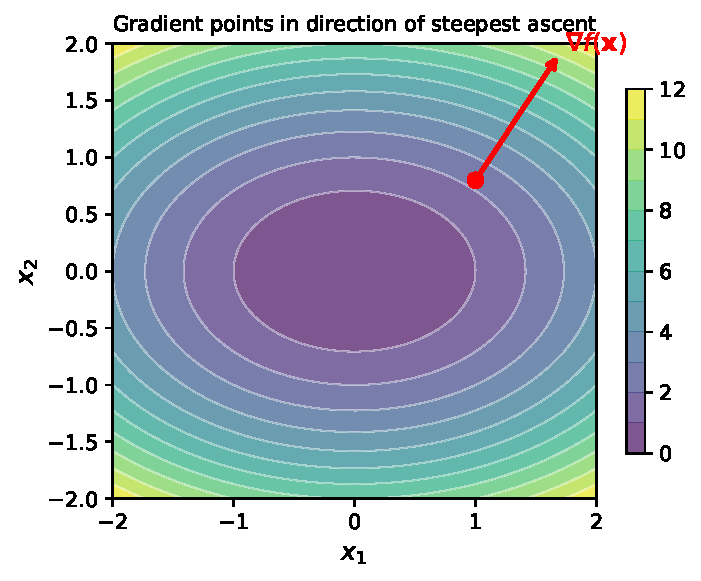
\includegraphics[width=\linewidth]{fig_gradient_contour.pdf}\\
    {\scriptsize Contour lines (level sets) of $f(x_1,x_2)=x_1^2+2x_2^2$.
     The gradient arrows are perpendicular to the contours and point
     outward toward higher values.}

    \column{0.47\linewidth}
    \textbf{Key geometric observations:}

    \medskip
    The gradient $\nabla f(\x)$ is always \emph{perpendicular} (orthogonal)
    to the level curve passing through $\x$.  Intuitively: if you stand on
    a hillside and look along a contour line, the steepest direction is
    exactly at right angles to it.

    \medskip
    Moving in the direction \emph{opposite} the gradient ---
    i.e., in the direction $-\nabla f(\x)$ --- is the direction of
    steepest descent.  Gradient-based minimizers update the current
    point $\x$ as:
    \[
      \x_{\text{new}} = \x - \alpha\,\nabla f(\x)
    \]
    where $\alpha$ (alpha) is a positive step size called the
    \emph{learning rate}.  We will revisit this update rule in detail
    when we study gradient descent methods.
  \end{columns}

\end{frame}

% ------------------------------------------------------------------------------
\begin{frame}[allowframebreaks]{The Jacobian Matrix}

  When a function has \emph{multiple outputs} --- not just a single
  number but a vector of numbers --- the natural generalization of the
  gradient is the \textbf{Jacobian matrix}.

  \begin{block}{Definition: Jacobian}
    For a function $\mathbf{f}:\mathbb{R}^n \to \mathbb{R}^m$ that maps
    an $n$-dimensional input vector to an $m$-dimensional output vector,
    the \textbf{Jacobian} $\mathbf{J}$ is the $m \times n$ matrix whose
    $(i,j)$-th entry is:
    \[
      \mathbf{J}_{ij} = \frac{\partial f_i}{\partial x_j}, \qquad
      \mathbf{J}
      =
      \begin{bmatrix}
        \dfrac{\partial f_1}{\partial x_1} & \cdots & \dfrac{\partial f_1}{\partial x_n}\\[8pt]
        \vdots & \ddots & \vdots\\[4pt]
        \dfrac{\partial f_m}{\partial x_1} & \cdots & \dfrac{\partial f_m}{\partial x_n}
      \end{bmatrix}
    \]
  \end{block}

  \begin{block}{Notation}
    \begin{itemize}
      \item $f_i$ is the $i$-th component of the output vector
            $\mathbf{f}(\x)$, for $i = 1, \ldots, m$.
      \item $x_j$ is the $j$-th component of the input vector $\x$,
            for $j = 1, \ldots, n$.
      \item $\mathbf{J}_{ij}$ (row $i$, column $j$) measures how the
            $i$-th output changes per unit change in the $j$-th input.
      \item ``$m \times n$ matrix'' means $m$ rows and $n$ columns.
    \end{itemize}
  \end{block}

  \framebreak

  \textbf{Special cases that connect to familiar objects:}

  \begin{itemize}
    \item When $m=1$ (scalar output), $\mathbf{f}$ is just an ordinary
          scalar function $f:\mathbb{R}^n\to\mathbb{R}$, and the Jacobian
          reduces to a $1\times n$ row vector equal to $\nabla f(\x)^\top$.
          So the gradient is just the Jacobian transposed.

    \item When $n=1$ (scalar input), the Jacobian is an $m\times 1$ column
          vector of ordinary scalar derivatives.
  \end{itemize}

  \medskip
  \textbf{Chain rule for vector functions.}
  Just as in one dimension, composed functions obey a chain rule.  If we
  have $\mathbf{h}(\x) = \mathbf{f}(\mathbf{g}(\x))$, then the Jacobian
  of the composition is the product of the Jacobians:
  \[
    \mathbf{J}_{\mathbf{h}} = \mathbf{J}_{\mathbf{f}} \cdot \mathbf{J}_{\mathbf{g}}.
  \]
  This matrix multiplication is the multi-dimensional generalization of
  multiplying scalar derivatives when applying the chain rule.  It is
  the core identity underlying automatic differentiation.

  \begin{exampleblock}{Worked Example}
    Let $\mathbf{f}(u,v) = (u+v,\; uv)^\top$ and
    $\mathbf{g}(x) = (x^2,\; x^3)^\top$.
    The Jacobian of $\mathbf{g}$ at $x=2$ is
    $\mathbf{J}_\mathbf{g} = \begin{bmatrix}2x\\3x^2\end{bmatrix}
    \big|_{x=2} = \begin{bmatrix}4\\12\end{bmatrix}$.
    The Jacobian of $\mathbf{f}$ at $(u,v)=(4,8)$ is
    $\mathbf{J}_\mathbf{f} = \begin{bmatrix}1&1\\v&u\end{bmatrix}
    = \begin{bmatrix}1&1\\8&4\end{bmatrix}$.
    By the chain rule:
    $\mathbf{J}_\mathbf{h} = \begin{bmatrix}1&1\\8&4\end{bmatrix}
    \begin{bmatrix}4\\12\end{bmatrix} = \begin{bmatrix}16\\64\end{bmatrix}$.
  \end{exampleblock}

\end{frame}

% ------------------------------------------------------------------------------
\begin{frame}[allowframebreaks]{The Hessian Matrix: Capturing Curvature}

  The gradient captures the \emph{first-order} (linear) behavior of $f$
  near a point.  For a better approximation --- and for understanding
  whether a critical point is a minimum, maximum, or saddle --- we need
  the \emph{second-order} (quadratic) information.  This is encoded by
  the \textbf{Hessian matrix}.

  \begin{columns}[T]
    \column{0.52\linewidth}
    \begin{block}{Definition: Hessian (eq.\ 2.8)}
      For a function $f:\mathbb{R}^n\to\mathbb{R}$, the \textbf{Hessian}
      $\mathbf{H}$ is the symmetric $n\times n$ matrix of all second-order
      partial derivatives:
      \[
        \mathbf{H}_{ij}
          = \frac{\partial^2 f}{\partial x_i\,\partial x_j}
      \]
      \[
        \mathbf{H}
        =
        \begin{bmatrix}
          f_{x_1 x_1} & \cdots & f_{x_1 x_n}\\
          \vdots & \ddots & \vdots\\
          f_{x_n x_1} & \cdots & f_{x_n x_n}
        \end{bmatrix}
      \]
    \end{block}

    \column{0.45\linewidth}
    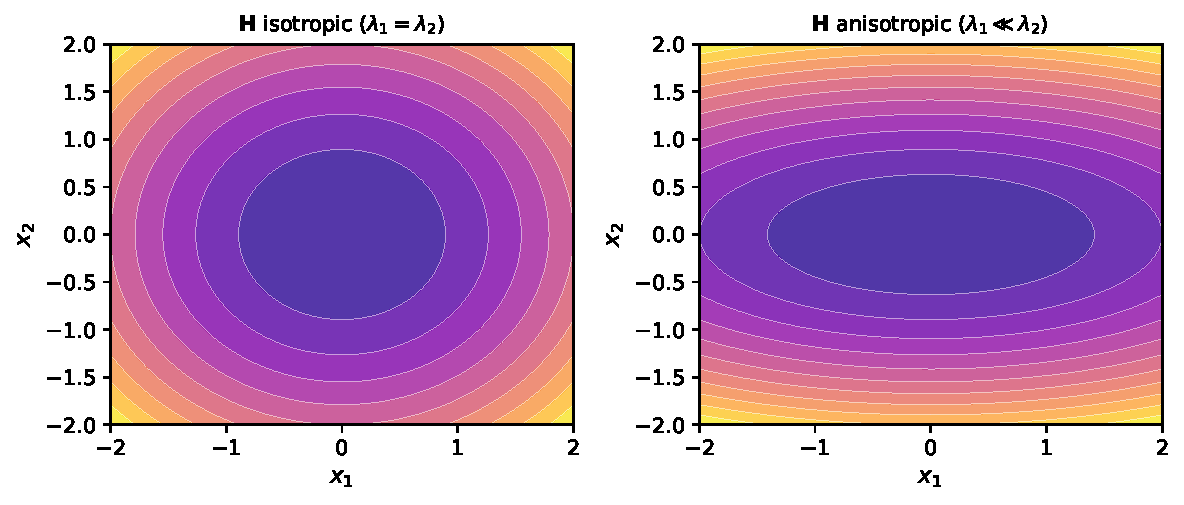
\includegraphics[width=\linewidth]{fig_hessian_curvature.pdf}\\
    {\scriptsize Top: isotropic curvature ($\lambda_1 = \lambda_2$, circular
    contours).  Bottom: anisotropic curvature --- the function curves much
    more steeply in one direction, producing elongated elliptical contours.}
  \end{columns}

  \framebreak

  \begin{block}{Notation}
    \begin{itemize}
      \item $\dfrac{\partial^2 f}{\partial x_i\,\partial x_j}$ (``second
            partial of $f$ with respect to $x_i$ then $x_j$'') means:
            first differentiate $f$ with respect to $x_j$ (holding all
            other variables fixed), then differentiate the result with
            respect to $x_i$.
      \item $f_{x_i x_j}$ is a compact shorthand for the same quantity.
      \item The diagonal entry $\mathbf{H}_{ii} = \partial^2 f / \partial x_i^2$
            is the ordinary second derivative with respect to $x_i$: it
            measures how the slope in the $x_i$ direction is itself changing.
      \item $\lambda$ (lambda) will denote eigenvalues of $\mathbf{H}$ in
            second-order analysis.
    \end{itemize}
  \end{block}

  \textbf{Symmetry.}
  Under mild smoothness conditions (Schwarz's theorem), the order of
  differentiation does not matter:
  $\mathbf{H}_{ij} = \mathbf{H}_{ji}$.
  So the Hessian is always a \emph{symmetric} matrix.

  \medskip
  \textbf{What the Hessian tells an optimizer.}
  The sign of the Hessian (more precisely, whether it is
  \emph{positive definite}) classifies critical points:
  if $\nabla f(\x)=\mathbf{0}$ and $\mathbf{H}$ is positive definite
  (all eigenvalues $> 0$), then $\x$ is a local minimum.
  If $\mathbf{H}$ is negative definite (all eigenvalues $< 0$), $\x$ is
  a local maximum.  If the eigenvalues have mixed signs, $\x$ is a saddle
  point.

  \medskip
  \textbf{The second-order Taylor approximation} of $f$ near $\x$:
  \[
    f(\x + \Delta\x)
    \;\approx\;
    f(\x)
    \;+\; \nabla f(\x)^\top \Delta\x
    \;+\; \tfrac{1}{2}\,\Delta\x^\top \mathbf{H}(\x)\,\Delta\x
  \]
  The last term $\tfrac{1}{2}\,\Delta\x^\top \mathbf{H}(\x)\,\Delta\x$
  is a \emph{quadratic form} (a generalization of $\tfrac{1}{2}f''(x)\,h^2$
  in 1-D) that captures the curvature.

  \begin{exampleblock}{Worked Example}
    Let $f(x_1,x_2) = x_1^2 + 3x_1 x_2 + 2x_2^2$.
    The first partial derivatives are $\partial f/\partial x_1 = 2x_1 + 3x_2$
    and $\partial f/\partial x_2 = 3x_1 + 4x_2$.
    The second partial derivatives are
    $f_{x_1 x_1} = 2$, $f_{x_1 x_2} = f_{x_2 x_1} = 3$,
    $f_{x_2 x_2} = 4$.
    So the Hessian is the constant matrix
    $\mathbf{H} = \begin{bmatrix}2 & 3\\ 3 & 4\end{bmatrix}$,
    which is symmetric.
  \end{exampleblock}

\end{frame}

% ------------------------------------------------------------------------------
\begin{frame}[allowframebreaks]{Directional Derivative}

  The gradient tells us the rate of change along each coordinate axis.
  But what if we want to know the rate of change along an \emph{arbitrary
  direction}?  That is the purpose of the \textbf{directional derivative}.

  \begin{block}{Definition: Directional Derivative (eq.\ 2.10)}
    The \textbf{directional derivative} of $f$ at $\x$ in the direction
    of a vector $\mathbf{s} \in \mathbb{R}^n$ is:
    \[
      \nabla_{\mathbf{s}} f(\x)
      \;=\;
      \lim_{h\to 0}\frac{f(\x + h\mathbf{s}) - f(\x)}{h}
      \;=\;
      \nabla f(\x)^\top \mathbf{s}
    \]
  \end{block}

  \begin{block}{Notation}
    \begin{itemize}
      \item $\mathbf{s}$ (``s bold'') is any nonzero direction vector.
            It is common to require $\|\mathbf{s}\| = 1$ (unit length) so
            that the directional derivative equals the actual slope
            (not scaled by the length of $\mathbf{s}$).
      \item $\nabla f(\x)^\top \mathbf{s}$ is the \emph{dot product}
            (inner product) of the gradient vector and the direction vector.
            For two vectors $\mathbf{a}$ and $\mathbf{b}$,
            $\mathbf{a}^\top \mathbf{b} = \|\mathbf{a}\|\|\mathbf{b}\|\cos\theta$
            where $\theta$ (theta) is the angle between them.
      \item $\mathbf{e}_i$ denotes the $i$-th standard basis vector
            (all zeros except a $1$ in position $i$).
    \end{itemize}
  \end{block}

  \begin{alertblock}{How to Read This Formula}
    Because $\nabla f(\x)^\top \mathbf{s}
    = \|\nabla f(\x)\|\,\|\mathbf{s}\|\cos\theta$,
    the directional derivative is largest when $\theta = 0$
    (i.e., $\mathbf{s}$ points in the same direction as $\nabla f(\x)$)
    and smallest (most negative) when $\theta = \pi$ (opposite direction).
    This confirms that the gradient itself is the direction of steepest
    ascent.
  \end{alertblock}

  \framebreak

  \textbf{Special cases.}
  If we choose $\mathbf{s} = \mathbf{e}_i$ (the $i$-th unit coordinate
  vector), then the directional derivative reduces to:
  \[
    \nabla_{\mathbf{e}_i} f(\x)
    = \nabla f(\x)^\top \mathbf{e}_i
    = \frac{\partial f}{\partial x_i}.
  \]
  So ordinary partial derivatives are just directional derivatives along
  coordinate axes.  The directional derivative is the unified concept.

  \medskip
  \begin{exampleblock}{Worked Numerical Example}
    Let $f(x_1,x_2) = x_1^2 + x_2^2$, evaluated at $\x=(1,1)^\top$.
    Choose direction $\mathbf{s} = \bigl(\tfrac{1}{\sqrt{2}},
    \tfrac{1}{\sqrt{2}}\bigr)^\top$ (the diagonal direction, which has
    unit length since $\|\mathbf{s}\| = \sqrt{(1/\sqrt{2})^2+(1/\sqrt{2})^2}=1$).

    Step 1: Compute the gradient.
    $\nabla f(x_1,x_2) = (2x_1,\,2x_2)^\top$,
    so $\nabla f(1,1) = (2,2)^\top$.

    Step 2: Compute the dot product.
    \[
      \nabla_\mathbf{s} f = (2,2) \cdot \left(\tfrac{1}{\sqrt{2}},\tfrac{1}{\sqrt{2}}\right)
      = 2\cdot\tfrac{1}{\sqrt{2}} + 2\cdot\tfrac{1}{\sqrt{2}}
      = \frac{2}{\sqrt{2}} + \frac{2}{\sqrt{2}}
      = 2\sqrt{2} \approx 2.83.
    \]
    This means: if we move in the diagonal direction from $(1,1)$, $f$
    increases at a rate of approximately $2.83$ per unit distance.
    For comparison, moving along the $x_1$-axis gives a rate of
    $\partial f/\partial x_1 = 2$, which is smaller.
  \end{exampleblock}

\end{frame}

% =============================================================================
\section{3. Numerical Differentiation}
% =============================================================================

\begin{frame}[allowframebreaks]{Finite Difference Methods: Overview and Intuition}

  When a function $f$ is available only as a piece of computer code --- not
  as an algebraic formula --- we cannot apply the rules of calculus directly.
  Instead, we can \emph{approximate} the derivative by evaluating $f$ at
  nearby points and measuring how much the output changes.  This family of
  approaches is called \textbf{finite difference approximation}.

  The idea is simply to replace the theoretical limit in the definition of the
  derivative with a small but nonzero step $h$:
  instead of taking $h \to 0$, we just pick a small value of $h$ and compute
  the ratio.  The error we introduce by not going all the way to zero is
  called the \emph{truncation error}.

  \begin{block}{The Three Finite Difference Approximations}
    \renewcommand{\arraystretch}{2.0}
    \begin{tabular}{lll}
      \toprule
      \textbf{Method} & \textbf{Formula} & \textbf{Truncation Error} \\
      \midrule
      Forward difference
        & $\dfrac{f(x+h)-f(x)}{h}$
        & $O(h)$ --- error proportional to $h$ \\
      Central difference
        & $\dfrac{f(x+h/2)-f(x-h/2)}{h}$
        & $O(h^2)$ --- error proportional to $h^2$ \\
      Backward difference
        & $\dfrac{f(x)-f(x-h)}{h}$
        & $O(h)$ --- error proportional to $h$ \\
      \bottomrule
    \end{tabular}
  \end{block}

  \begin{alertblock}{How to Read the Error Column}
    ``$O(h)$'' (pronounced ``big-O of h'') means the error is roughly
    proportional to $h$: halving $h$ halves the error.
    ``$O(h^2)$'' means the error is proportional to $h^2$: halving $h$
    \emph{quarters} the error.  So central difference converges much faster
    as $h$ decreases --- it is second-order accurate while forward and
    backward are only first-order accurate.
  \end{alertblock}

\end{frame}

% ------------------------------------------------------------------------------
\begin{frame}[allowframebreaks]{Forward Difference: Taylor Series Analysis}

  To understand \emph{why} the forward difference approximation has an
  $O(h)$ error, we use the \textbf{Taylor series} expansion of $f$ around
  the point $x$.

  \begin{block}{Taylor Expansion of $f(x+h)$ around $x$}
    For any smooth function $f$:
    \[
      f(x+h)
      = f(x)
      + f'(x)\,h
      + \frac{f''(x)}{2!}\,h^2
      + \frac{f'''(x)}{3!}\,h^3
      + \cdots
    \]
  \end{block}

  \begin{block}{Notation}
    \begin{itemize}
      \item $f''(x)$ (``f double-prime of x'') is the second derivative
            of $f$ at $x$: it measures the rate of change of the slope.
      \item $f'''(x)$ (``f triple-prime of x'') is the third derivative.
      \item $2! = 2 \times 1 = 2$ and $3! = 3 \times 2 \times 1 = 6$
            are factorial numbers (the ``$!$'' symbol means factorial).
      \item The dots ($\cdots$) indicate higher-order terms that become
            negligible as $h \to 0$.
    \end{itemize}
  \end{block}

  Rearranging the expansion to isolate $f'(x)$:
  \[
    f'(x)
    = \frac{f(x+h) - f(x)}{h}
    \underbrace{- \frac{f''(x)}{2}\,h - \frac{f'''(x)}{6}\,h^2 - \cdots}_{\text{truncation error}}
  \]

  The forward difference formula drops all the error terms, keeping only
  the first fraction.  The dominant error term is $-\dfrac{f''(x)}{2}\,h$,
  which is proportional to $h$.  This confirms the $O(h)$ accuracy.

  \framebreak

  \textbf{The step-size dilemma.}
  You might think: simply make $h$ very small and the error disappears.
  Unfortunately, there is a competing source of error: \emph{floating-point
  round-off}.

  When $h$ is so small that $f(x+h)$ and $f(x)$ are nearly equal, their
  difference $f(x+h) - f(x)$ is computed by subtracting two nearly
  identical numbers.  In floating-point arithmetic, this causes
  \emph{subtractive cancellation}: the significant digits cancel and
  the result is dominated by rounding error.

  \begin{columns}[T]
    \column{0.50\linewidth}
    \textbf{Two competing errors:}
    \begin{itemize}
      \item \textbf{Truncation error} ($\propto h$): decreases as $h$ shrinks.
      \item \textbf{Round-off error} ($\propto 1/h$ approximately): grows as
            $h$ shrinks.
    \end{itemize}
    There is an \emph{optimal} $h$ that balances the two.

    \column{0.47\linewidth}
    \textbf{Practical recommendation:}
    For forward difference in 64-bit floating-point arithmetic (where the
    machine epsilon $\epsilon_{\text{mach}} \approx 2.2 \times 10^{-16}$),
    the optimal step size is approximately:
    \[
      h \approx \sqrt{\epsilon_{\text{mach}}} \approx 10^{-8}
    \]
    Using $h$ much smaller than this will \emph{increase} the total error
    due to cancellation.
  \end{columns}

\end{frame}

% ------------------------------------------------------------------------------
\begin{frame}[allowframebreaks]{Central Difference: Why It Is More Accurate}

  The central difference formula uses symmetric points on both sides of $x$
  and achieves $O(h^2)$ accuracy rather than $O(h)$.  Here is why.

  We expand both $f(x+h/2)$ and $f(x-h/2)$ using Taylor's theorem:

  \begin{block}{Two Taylor Expansions}
    \[
      f\!\left(x+\tfrac{h}{2}\right)
      = f(x) + f'(x)\tfrac{h}{2}
      + \frac{f''(x)}{2}\!\left(\tfrac{h}{2}\right)^{\!2}
      + \frac{f'''(x)}{6}\!\left(\tfrac{h}{2}\right)^{\!3} + \cdots
    \]
    \[
      f\!\left(x-\tfrac{h}{2}\right)
      = f(x) - f'(x)\tfrac{h}{2}
      + \frac{f''(x)}{2}\!\left(\tfrac{h}{2}\right)^{\!2}
      - \frac{f'''(x)}{6}\!\left(\tfrac{h}{2}\right)^{\!3} + \cdots
    \]
  \end{block}

  Now subtract the second equation from the first.  Notice that every
  term with an \emph{even power of $h$} cancels (because the
  $(\cdot)^2$ terms are identical), and every term with an
  \emph{odd power of $h$} survives but with coefficient doubled:

  \[
    f\!\left(x+\tfrac{h}{2}\right) - f\!\left(x-\tfrac{h}{2}\right)
    = f'(x)\,h + \frac{f'''(x)}{6}\cdot\frac{h^3}{4} + \cdots
  \]

  Dividing by $h$:
  \[
    f'(x)
    = \frac{f(x+h/2) - f(x-h/2)}{h}
    - \frac{f'''(x)}{24}\,h^2
    + \cdots
  \]

  The leading error term is now $O(h^2)$: the even-order (second-derivative)
  term has cancelled out exactly, leaving only the third-derivative term.

  \begin{alertblock}{Key Insight}
    The cancellation of even-order terms is the reason central differences
    are more accurate.  The error drops as $h^2$ rather than $h$, so
    reducing $h$ by a factor of 10 reduces the error by a factor of 100.
    The optimal step size for central difference is approximately
    $h \approx \epsilon_{\text{mach}}^{1/3} \approx 10^{-5}$.
  \end{alertblock}

\end{frame}

% ------------------------------------------------------------------------------
\begin{frame}[fragile]{Finite Difference: Python Implementation}
\begin{lstlisting}[caption={Forward, central, and backward finite difference --- Python (NumPy)}]
import numpy as np

def diff_forward(f, x, h=1e-8):
    """Forward difference: O(h) error. Use h ~ sqrt(eps_machine)."""
    return (f(x + h) - f(x)) / h

def diff_central(f, x, h=1e-5):
    """Central difference: O(h^2) error. Use h ~ eps_machine^(1/3)."""
    return (f(x + h/2) - f(x - h/2)) / h

def diff_backward(f, x, h=1e-8):
    """Backward difference: O(h) error."""
    return (f(x) - f(x - h)) / h

# Gradient for multivariate f: R^n -> R  (central difference per component)
def gradient_fd(f, x, h=1e-5):
    """Numerical gradient using central differences along each axis."""
    n = len(x)
    g = np.zeros(n)
    for i in range(n):
        xp, xm = x.copy(), x.copy()
        xp[i] += h/2;  xm[i] -= h/2
        g[i] = (f(xp) - f(xm)) / h
    return g

# Running example: f(x) = sin(x^2), x = pi/2
f = lambda x: np.sin(x**2)
x0 = np.pi / 2
true_val = 2*x0 * np.cos(x0**2)   # chain rule: 2x * cos(x^2)
print(f"True:    {true_val:.8f}")
print(f"Forward: {diff_forward(f, x0):.8f}")
print(f"Central: {diff_central(f, x0):.8f}")
\end{lstlisting}
\end{frame}

% ------------------------------------------------------------------------------
\begin{frame}[allowframebreaks]{Finite Difference: Visual Comparison}

  The figure below illustrates how the three finite difference methods
  relate geometrically to the true tangent.

  \centering
  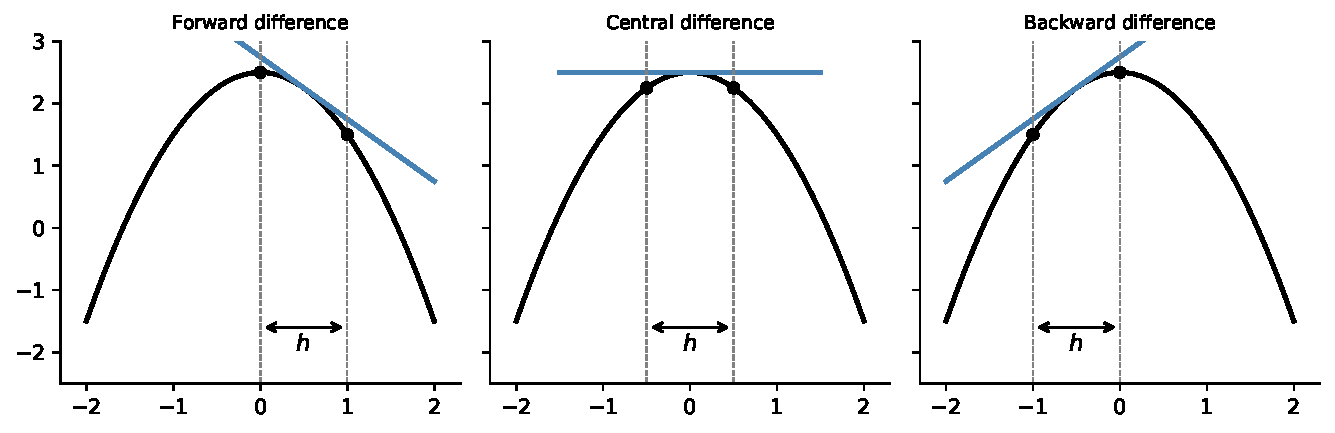
\includegraphics[width=0.60\linewidth]{fig_differences.pdf}

  \raggedright
  \medskip
  \textbf{Reading the figure.}
  All three methods approximate the tangent slope (the true derivative,
  shown as the blue tangent line) by the slope of a secant line connecting
  two points on the curve:
  \begin{itemize}
    \item \textbf{Forward difference} connects $(x, f(x))$ and
          $(x+h, f(x+h))$ --- a secant leaning to the right.
    \item \textbf{Backward difference} connects $(x-h, f(x-h))$ and
          $(x, f(x))$ --- a secant leaning to the left.
    \item \textbf{Central difference} connects $(x-h/2, f(x-h/2))$ and
          $(x+h/2, f(x+h/2))$ --- a symmetric secant centered on $x$.
          Because it is symmetric, it inherits the same slope error
          cancellation we derived above, giving $O(h^2)$ accuracy.
  \end{itemize}

\end{frame}

% ------------------------------------------------------------------------------
\begin{frame}[allowframebreaks]{The Complex-Step Method: Avoiding Cancellation}

  Finite differences suffer from a fundamental tension: smaller $h$ reduces
  the truncation error but amplifies the round-off error from subtractive
  cancellation.  The \textbf{complex-step method} cleverly eliminates this
  cancellation entirely by evaluating $f$ at a \emph{complex} argument.

  \begin{block}{Core Idea}
    Instead of comparing two real evaluations, evaluate $f$ at the
    complex point $x + ih$, where $i = \sqrt{-1}$ is the imaginary unit
    and $h$ is a small real number.
  \end{block}

  Expanding $f(x+ih)$ in a Taylor series (treating $ih$ as the small
  perturbation):
  \[
    f(x+ih)
    = f(x)
    + ih\,f'(x)
    + \frac{(ih)^2}{2!} f''(x)
    + \frac{(ih)^3}{3!} f'''(x)
    + \cdots
  \]
  Using $i^2 = -1$ and $i^3 = -i$:
  \[
    f(x+ih)
    = \underbrace{f(x) - \tfrac{h^2}{2} f''(x) + \cdots}_{\text{Real part}}
    +\; i\underbrace{\left(h f'(x) - \tfrac{h^3}{6} f'''(x) + \cdots\right)}_{\text{Imaginary part}}
  \]

  Taking the imaginary part and dividing by $h$:
  \[
    \boxed{f'(x)
    \approx \frac{\operatorname{Im}(f(x+ih))}{h} + O(h^2)}
  \]

  \framebreak

  \begin{block}{Notation}
    \begin{itemize}
      \item $i$ is the imaginary unit satisfying $i^2 = -1$.  A complex
            number is any number of the form $a + bi$ where $a$ and $b$
            are real numbers.
      \item $\operatorname{Im}(\cdot)$ (``imaginary part of'') extracts
            the $b$ from $a + bi$.
      \item $\operatorname{Re}(\cdot)$ (``real part of'') extracts $a$.
    \end{itemize}
  \end{block}

  \begin{alertblock}{Why There Is No Cancellation}
    In finite differences we compute $f(x+h) - f(x)$ --- a subtraction
    of two nearly equal numbers, which destroys precision.  In the
    complex-step method we extract the \emph{imaginary part} of a single
    function evaluation.  Imaginary and real parts do not cancel each
    other, so there is no subtractive cancellation.  This means we can
    safely use $h = 10^{-20}$ or even smaller, obtaining near-machine-precision
    derivatives.
  \end{alertblock}

  \textbf{Requirement.}  The function $f$ must be able to accept a complex
  number as input and produce a complex number as output.  This is
  called being \emph{analytic} (or holomorphic).  Most mathematical
  functions (polynomials, $\sin$, $\exp$, $\ln$, etc.) are analytic.
  NumPy handles complex arrays transparently, so Python code written
  with NumPy usually works without modification.

\end{frame}

% ------------------------------------------------------------------------------
\begin{frame}[fragile]{Complex-Step Method: Python Code and Example}
\begin{lstlisting}[caption={Complex-step derivative --- Python (NumPy complex arithmetic)}]
import numpy as np

def diff_complex(f, x, h=1e-20):
    """
    Complex-step derivative: Im( f(x + i*h) ) / h
    No subtractive cancellation: h can be made arbitrarily small.
    """
    return np.imag(f(x + h * 1j)) / h

# Example: f(x) = sin(x^2)
# True derivative by chain rule: f'(x) = 2x * cos(x^2)
f = lambda x: np.sin(x**2)
x0 = np.pi / 2

# A single complex evaluation gives BOTH f(x0) and f'(x0)
v = f(x0 + 1e-20j)
fx   = np.real(v)          # f(x0) ~ 0.62426
dfdx = np.imag(v) / 1e-20  # f'(x0)

print(f"f(pi/2)  = {fx:.8f}")
print(f"f'(pi/2) = {dfdx:.8f}")

# True derivative: 2*(pi/2)*cos((pi/2)^2) = pi * cos(pi^2/4)
true_d = np.pi * np.cos(np.pi**2 / 4)
print(f"True     = {true_d:.8f}")
# Both complex-step and true agree to all 8 decimal places shown.
\end{lstlisting}

\medskip
Note that a \emph{single} function call provides both $f(x_0)$ (real part)
and $f'(x_0)$ (imaginary part divided by $h$).
\end{frame}

% ------------------------------------------------------------------------------
\begin{frame}[allowframebreaks]{Error Comparison: Forward vs.\ Central vs.\ Complex-Step}

  \begin{columns}[T]
    \column{0.53\linewidth}
    \centering
    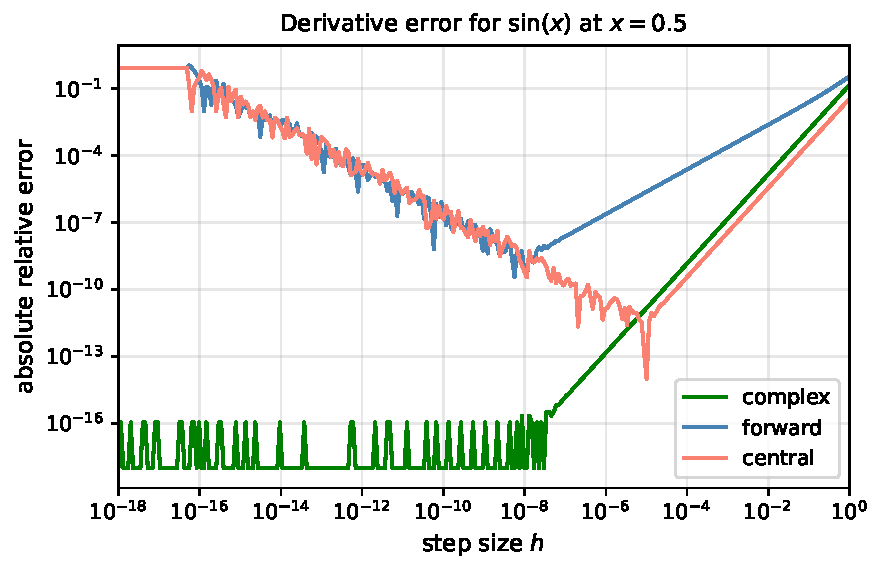
\includegraphics[width=\linewidth]{fig_error_comparison.pdf}

    \column{0.44\linewidth}
    \textbf{Reading the log-log error plot.}

    The horizontal axis shows the step size $h$ on a logarithmic scale
    (each tick is a power of 10), and the vertical axis shows the
    absolute error in the derivative estimate, also on a logarithmic scale.

    \medskip
    \textbf{Forward difference} (blue): the error decreases linearly
    (slope $-1$ on a log-log plot, confirming $O(h)$) until $h$ becomes
    so small that round-off dominates, after which the error rises.

    \medskip
    \textbf{Central difference} (orange): decreases with slope $-2$
    (confirming $O(h^2)$), hitting a floor at a smaller error before
    round-off takes over.

    \medskip
    \textbf{Complex-step} (green): stays flat near machine precision for
    all small $h$ --- there is no round-off floor because there is no
    subtraction.
  \end{columns}

  \begin{alertblock}{Key Takeaway}
    If your function supports complex inputs (which NumPy functions do),
    always prefer the complex-step method: it achieves near-machine-precision
    accuracy and requires exactly the same number of function evaluations
    (one) as forward difference, but without any step-size tuning.
  \end{alertblock}

\end{frame}

% =============================================================================
\section{4. Automatic Differentiation}
% =============================================================================

\begin{frame}[allowframebreaks]{Automatic Differentiation: The Best of Both Worlds}

  We have seen three approaches so far:
  \begin{itemize}
    \item \textbf{Symbolic differentiation} gives exact derivatives but
          requires the function to have an algebraic formula and can suffer
          from expression swell.
    \item \textbf{Finite differences} are easy to implement but approximate,
          with accuracy limited by step-size trade-offs.
    \item \textbf{Complex-step} eliminates cancellation but still requires
          the function to support complex inputs.
  \end{itemize}

  \textbf{Automatic differentiation (AD)} is a fourth approach that combines
  the best of symbolic and numerical methods: it computes \emph{exact}
  (up to floating-point precision) derivatives of a function given as
  computer code, without needing a closed-form formula and without any
  step-size approximation.

  \medskip
  The key insight is that any computer program is composed of a finite
  sequence of \emph{elementary operations} --- addition, subtraction,
  multiplication, division, $\sin$, $\exp$, $\ln$, etc. --- each of which
  has a known derivative.  By applying the \textbf{chain rule}
  systematically through the sequence of operations, AD computes the
  derivative of the whole program.

  \begin{block}{Chain Rule (the Engine of AD)}
    If $f = f(g(x))$, then:
    \[
      \frac{d}{dx}\,f(g(x))
      = \frac{df}{dg} \cdot \frac{dg}{dx}
    \]
  \end{block}

  \begin{block}{Notation}
    \begin{itemize}
      \item $g(x)$ is an intermediate value computed on the way to $f$.
      \item $\dfrac{df}{dg}$ (``d-f over d-g'') is the derivative of the
            outer function with respect to its input $g$.
      \item $\dfrac{dg}{dx}$ (``d-g over d-x'') is the derivative of the
            inner function with respect to $x$.
      \item The chain rule says these two local slopes multiply to give
            the overall slope.
    \end{itemize}
  \end{block}

  \framebreak

  \textbf{The computational graph.}
  Every program can be represented as a \textbf{directed acyclic graph}
  (DAG) where each node is an elementary operation and each edge
  carries a value from one operation to the next.  This is called the
  \emph{computational graph}.

  \begin{columns}[T]
    \column{0.52\linewidth}
    \centering
    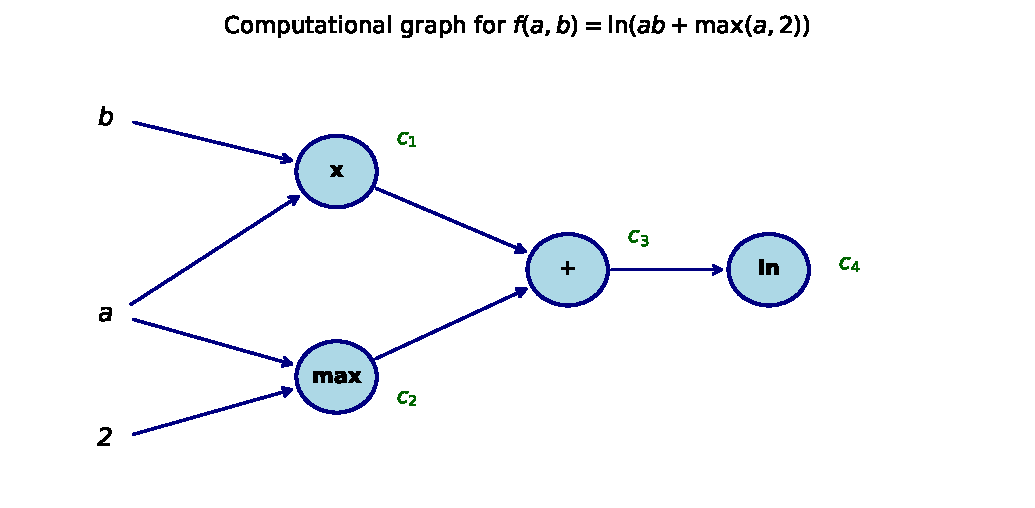
\includegraphics[width=0.95\linewidth]{fig_comp_graph.pdf}\\
    {\scriptsize Computational graph for
    $f(a,b)=\ln(ab+\max(a,2))$.}

    \column{0.45\linewidth}
    The graph for $f(a,b)=\ln(ab+\max(a,2))$ has:
    \begin{itemize}
      \item \textbf{Leaf nodes} (inputs): $a$, $b$, and the constant $2$.
      \item \textbf{Internal nodes} (operations):
            $c_1 = a \times b$,\quad
            $c_2 = \max(a, 2)$,\quad
            $c_3 = c_1 + c_2$,\quad
            $c_4 = \ln(c_3)$.
      \item \textbf{Terminal node} (output): $c_4 = f(a,b)$.
    \end{itemize}
    There are two strategies to traverse this graph and accumulate
    derivatives: \textbf{forward accumulation} (from inputs to output)
    and \textbf{reverse accumulation} (from output back to inputs).
  \end{columns}

\end{frame}

% ------------------------------------------------------------------------------
\begin{frame}[allowframebreaks]{Forward Accumulation (Forward Mode AD)}

  \textbf{Idea.}
  Traverse the computational graph from inputs to output, computing
  at each node both the function value and the derivative of that
  intermediate value with respect to a chosen input variable.
  We call these derivative values \emph{tangents} or \emph{dots}
  and write $\dot{c}_i = \partial c_i / \partial x$ for a chosen
  input $x$.

  \begin{block}{Forward Mode Chain Rule}
    At each node $c_i$ that depends on parent nodes $c_j$:
    \[
      \dot{c}_i = \frac{\partial c_i}{\partial c_j} \cdot \dot{c}_j
                  \quad\text{(accumulated over all parent nodes)}
    \]
    Seed: set $\dot{x} = 1$ for the input variable of interest and
    $\dot{y} = 0$ for all other inputs.
  \end{block}

  \textbf{Worked Example (eq.\ 2.26--2.30).}
  Compute $\partial f / \partial a$ for $f(a,b) = \ln(ab + \max(a,2))$
  at $a=3$, $b=2$.  Seed: $\dot{a} = 1$, $\dot{b} = 0$.

  \begin{columns}[T]
    \column{0.50\linewidth}
    \small
    \begin{tabular}{llll}
      \toprule
      \textbf{Node} & \textbf{Value} & \textbf{Derivative $\dot{c}$} & \textbf{Why} \\
      \midrule
      $a$ & $3$ & $\dot{a}=1$ & seed \\
      $b$ & $2$ & $\dot{b}=0$ & seed \\
      $c_1=ab$ & $6$ & $b\dot{a}+a\dot{b}=2$ & product rule \\
      $c_2=\max(a,2)$ & $3$ & $\dot{a}=1$ & $a>2$ \\
      $c_3=c_1+c_2$ & $9$ & $\dot{c}_1+\dot{c}_2=3$ & sum rule \\
      $c_4=\ln c_3$ & $\ln 9$ & $\dot{c}_3/c_3=3/9=1/3$ & log rule \\
      \bottomrule
    \end{tabular}

    \column{0.47\linewidth}
    \textbf{Result:}
    \[
      f(3,2) = \ln 9 \approx 2.197
      \qquad
      \frac{\partial f}{\partial a}\bigg|_{(3,2)} = \frac{1}{3}
    \]
    \textbf{Cost:} One forward pass computes the value of $f$ and the
    derivative with respect to \emph{one} input.  To compute the full
    gradient (derivatives with respect to $a$ \emph{and} $b$), we need
    two forward passes --- one with seed $(\dot{a},\dot{b})=(1,0)$ and
    one with $(0,1)$.  In general, for $n$ inputs we need $n$ passes.
    Forward mode is therefore efficient when $n$ is small.
  \end{columns}

  \framebreak

  \textbf{Dual numbers: an elegant implementation of forward mode.}

  A \textbf{dual number} is a pair $(a, b)$ written as $a + b\epsilon$
  (epsilon), where $\epsilon$ (``epsilon'') is an abstract symbol with
  the special property $\epsilon^2 = 0$ (but $\epsilon \neq 0$).

  The value $a$ stores the function value, and $b$ stores the derivative.
  Dual number arithmetic automatically propagates both simultaneously:

  \begin{block}{Dual Number Arithmetic (eq.\ 2.32--2.33)}
    \begin{align*}
      (a+b\epsilon) + (c+d\epsilon) &= (a+c) + (b+d)\epsilon \\
      (a+b\epsilon) \times (c+d\epsilon)
        &= (ac) + (ad+bc)\epsilon + \underbrace{bd\epsilon^2}_{=0}
         = (ac) + (ad+bc)\epsilon
    \end{align*}
  \end{block}

  The multiplication rule $(ad+bc)$ is exactly the product rule from
  calculus: if $c_1 = a \cdot b$ then $\dot{c}_1 = \dot{a}b + a\dot{b}$.
  So dual number arithmetic encodes the chain rule for free.

  \medskip
  To compute $f'(x_0)$: initialize $x = x_0 + 1\cdot\epsilon$ and run
  $f$ normally.  The $\epsilon$-coefficient of the output is $f'(x_0)$.

\end{frame}

% ------------------------------------------------------------------------------
\begin{frame}[fragile]{Forward AD: Python Implementation with Dual Numbers}
\begin{lstlisting}[caption={Dual number class implementing forward-mode automatic differentiation}]
import numpy as np

class Dual:
    """A dual number v + d*eps, where eps^2 = 0.
    v holds the function value; d holds the derivative."""
    def __init__(self, v, d=0.0):
        self.v, self.d = float(v), float(d)

    def __add__(self, other):
        if isinstance(other, Dual):
            return Dual(self.v + other.v, self.d + other.d)
        return Dual(self.v + other, self.d)        # add scalar constant
    __radd__ = __add__

    def __mul__(self, other):
        if isinstance(other, Dual):
            # product rule: (a+b*eps)*(c+d*eps) = ac + (ad+bc)*eps
            return Dual(self.v * other.v,
                        self.v * other.d + self.d * other.v)
        return Dual(self.v * other, self.d * other)
    __rmul__ = __mul__

    def log(self):
        # d/dx ln(x) = 1/x, so chain rule gives: derivative = self.d / self.v
        return Dual(np.log(self.v), self.d / self.v)

# Example: f(a,b) = log(a*b + max(a, 2)) at a=3, b=2
def f(a, b):
    c1 = a * b
    c2 = Dual(max(a.v, 2), a.d if a.v > 2 else 0.0)  # max is piecewise
    return (c1 + c2).log()

a = Dual(3.0, 1.0)   # seed: differentiating w.r.t. a
b = Dual(2.0, 0.0)   # b is held constant
result = f(a, b)
print(f"f(3,2)  = {result.v:.6f}")   # ln(9) ~ 2.197225
print(f"df/da   = {result.d:.6f}")   # 1/3   ~ 0.333333
\end{lstlisting}
\end{frame}

% ------------------------------------------------------------------------------
\begin{frame}[allowframebreaks]{Reverse Accumulation (Backpropagation)}

  While forward mode computes derivatives one input at a time,
  \textbf{reverse mode} computes derivatives with respect to
  \emph{all inputs simultaneously} in a single backward pass.
  This makes it the method of choice when there are many inputs and
  few outputs --- the standard situation in machine learning, where
  $f$ is a scalar loss function of millions of parameters.

  \medskip
  \textbf{The idea.}
  Define the \textbf{adjoint} (sensitivity) of each intermediate value
  $c_i$ as:
  \[
    \bar{c}_i = \frac{\partial f}{\partial c_i}
  \]
  This measures how much the final output $f$ would change if $c_i$
  changed by a small amount.  The output node has adjoint
  $\bar{c}_{\text{output}} = 1$ (changing the output by 1 changes $f$
  by 1).

  \begin{block}{Reverse Mode Propagation Rule}
    For each node $c_i$ with children $c_j$ (nodes that use $c_i$):
    \[
      \bar{c}_i
      = \sum_{j:\,j\text{ uses }i}
        \bar{c}_j \cdot \frac{\partial c_j}{\partial c_i}
    \]
  \end{block}

  \begin{block}{Notation}
    \begin{itemize}
      \item $\bar{c}_i$ (``c-bar sub-i'', read as ``adjoint of $c_i$'')
            is the sensitivity of the output to the intermediate value $c_i$.
      \item The sum runs over all nodes $c_j$ that directly depend on $c_i$
            in the computational graph.
      \item $\dfrac{\partial c_j}{\partial c_i}$ is the local derivative
            of the operation at node $c_j$ with respect to its input $c_i$.
    \end{itemize}
  \end{block}

  \framebreak

  \textbf{Two-phase procedure.}
  \begin{enumerate}
    \item \textbf{Forward pass}: run the program normally to compute
          all intermediate values $c_i$ and the output $f$.  Store
          (``tape'') all intermediate values needed for the backward pass.
    \item \textbf{Backward pass}: propagate adjoints from the output back
          to the inputs, applying the rule above at each node.
  \end{enumerate}

  The backward pass costs approximately 2--3 times a single forward pass,
  regardless of the number of inputs $n$.  So the total cost is about
  $3\times$ a forward evaluation to get the \emph{full gradient} with
  respect to all $n$ inputs simultaneously.  For neural networks with
  millions of parameters, this is an enormous saving over forward mode
  (which would need $n$ forward passes).

  \begin{block}{Forward vs.\ Reverse Mode Comparison}
    \renewcommand{\arraystretch}{1.4}
    \begin{tabular}{lll}
      \toprule
      & \textbf{Forward mode} & \textbf{Reverse mode (backprop)} \\
      \midrule
      Passes needed & $n$ (one per input) & $m$ (one per output) \\
      Best when & $n \ll m$ (few inputs) & $m \ll n$ (few outputs) \\
      Memory cost & $O(1)$ & $O(\text{graph size})$ --- must store tape \\
      Deep learning & less common & \textbf{this is backpropagation} \\
      \bottomrule
    \end{tabular}
  \end{block}

  \textbf{The deep learning connection.}
  In deep learning, the function $f:\mathbb{R}^n \to \mathbb{R}$ is the
  scalar training loss and $n$ is the number of model parameters
  (potentially billions).  Reverse mode (backpropagation) computes the
  full gradient $\nabla f$ in a single backward pass --- this is why
  training large neural networks is computationally feasible at all.

\end{frame}

% ------------------------------------------------------------------------------
\begin{frame}[fragile]{Reverse AD in Practice: Using JAX}
\begin{lstlisting}[caption={Automatic differentiation with JAX --- both forward and reverse mode}]
# Install: pip install jax
import jax
import jax.numpy as jnp

# Define a function with two inputs
def f(x):
    # f(a, b) = ln(a*b + max(a, 2.0))
    return jnp.log(x[0]*x[1] + jnp.maximum(x[0], 2.0))

x0 = jnp.array([3.0, 2.0])

# --- Reverse mode: full gradient in one backward pass ---
grad_f = jax.grad(f)          # grad_f is a function that returns the gradient
g = grad_f(x0)                # [df/da, df/db]
print(f"df/da = {g[0]:.4f}")  # expected: 0.3333
print(f"df/db = {g[1]:.4f}")  # expected: 0.3333

# --- Forward mode: Jacobian-vector product ---
# jax.jvp computes (f(x0), J(x0) * v) where v is a tangent vector
primals, tangents = jax.jvp(f, (x0,), (jnp.array([1.0, 0.0]),))
print(f"f(3,2) = {primals:.4f}")       # ~2.1972
print(f"df/da via JVP = {tangents:.4f}")  # 0.3333

# --- Hessian via nested AD ---
hess = jax.hessian(f)(x0)
print("Hessian:\n", hess)
\end{lstlisting}

\medskip
JAX's \texttt{jax.grad} uses reverse mode; \texttt{jax.jvp} uses forward
mode.  Both give exact (floating-point) derivatives of the Python/NumPy
function without any finite difference approximation.
\end{frame}

% =============================================================================
\section{5. Regression Gradient}
% =============================================================================

\begin{frame}[allowframebreaks]{Regression Gradient: Estimating Gradients for Black-Box Functions}

  All the methods discussed so far --- symbolic, finite difference,
  complex-step, and automatic differentiation --- require some form of
  access to the internals of $f$: either its algebraic formula (symbolic,
  AD) or the ability to evaluate it at complex arguments (complex-step).

  \textbf{What if $f$ is a true black box?}
  For example, $f$ might be a physical simulation, an experiment, or a
  proprietary software tool that can only be queried at real-valued inputs.
  In that case, we can estimate the gradient using only real-valued
  function evaluations, by treating gradient estimation as a
  \emph{linear regression problem}.

  \medskip
  \textbf{The idea.}
  Near any point $\x$, the first-order Taylor approximation says:
  \[
    f(\x + \Delta\x) \approx f(\x) + \mathbf{g}^\top \Delta\x
  \]
  where $\mathbf{g}$ (``g bold'') is the gradient we want to estimate.
  If we evaluate $f$ at $m$ perturbed points
  $\x + \Delta\x^{(1)}, \ldots, \x + \Delta\x^{(m)}$,
  we get $m$ approximate equations of this form.
  We can then find the $\mathbf{g}$ that best fits all these equations
  simultaneously --- that is, solve a least-squares regression problem.

  \begin{block}{The Optimization Problem (eq.\ 2.42)}
    Find the vector $\mathbf{g} \in \mathbb{R}^n$ minimizing the sum of
    squared fitting errors:
    \[
      \min_{\mathbf{g}} \sum_{i=1}^{m}
      \left(
        f\!\left(\x + \Delta\x^{(i)}\right)
        - \left(f(\x) + \mathbf{g}^\top \Delta\x^{(i)}\right)
      \right)^{\!2}
    \]
  \end{block}

  \begin{block}{Notation}
    \begin{itemize}
      \item $\Delta\x^{(i)}$ (``Delta x superscript i''; the superscript
            in parentheses is an \emph{index}, not a power) is the $i$-th
            perturbation vector: the direction and distance we moved
            $\x$ to get the $i$-th sample point.
      \item $m$ is the number of perturbation samples.
      \item $\sum_{i=1}^{m}$ (Sigma, ``sum from $i$ equals one to $m$'')
            means we add up the squared errors for all $m$ perturbations.
      \item $\mathbf{g}^\top \Delta\x^{(i)}$ is the predicted change in
            $f$ according to the linear model.
    \end{itemize}
  \end{block}

  \framebreak

  \begin{block}{Matrix Formulation and Closed-Form Solution (eq.\ 2.43--2.46)}
    Stack the perturbations into a matrix and the function differences
    into a vector:
    \[
      \Delta\mathbf{X}
      =
      \begin{bmatrix}
        (\Delta\x^{(1)})^\top \\
        \vdots \\
        (\Delta\x^{(m)})^\top
      \end{bmatrix}
      \in \mathbb{R}^{m\times n},
      \qquad
      \Delta\mathbf{f}
      =
      \begin{bmatrix}
        f(\x+\Delta\x^{(1)})-f(\x) \\
        \vdots \\
        f(\x+\Delta\x^{(m)})-f(\x)
      \end{bmatrix}
      \in \mathbb{R}^m
    \]
    The minimization problem becomes a standard least-squares problem:
    $\min_{\mathbf{g}} \|\Delta\mathbf{X}\,\mathbf{g} - \Delta\mathbf{f}\|^2$.
    The closed-form solution is:
    \[
      \boxed{\mathbf{g} = \Delta\mathbf{X}^{+}\,\Delta\mathbf{f}}
    \]
    where $\Delta\mathbf{X}^{+}$ (``Delta X pseudoinverse'') is the
    \textbf{Moore-Penrose pseudoinverse} of $\Delta\mathbf{X}$.
  \end{block}

  \begin{alertblock}{How to Read This Formula}
    The pseudoinverse $\Delta\mathbf{X}^{+}$ is a generalization of the
    ordinary matrix inverse that works even when $\Delta\mathbf{X}$ is
    not square (we typically have $m > n$ so there are more equations
    than unknowns).  It finds the least-squares solution automatically.
    In practice, use \texttt{np.linalg.lstsq} rather than explicitly
    computing the pseudoinverse.
  \end{alertblock}

  \textbf{Generating perturbations.}
  Draw each $\Delta\x^{(i)}$ uniformly from a hypersphere of radius
  $\delta$ (delta) centered at the origin.  This ensures the perturbations
  uniformly cover all directions so the regression is well-conditioned.

\end{frame}

% ------------------------------------------------------------------------------
\begin{frame}[fragile]{Regression Gradient: Python Implementation}
\begin{lstlisting}[caption={Regression gradient estimator (Algorithm 2.3 in Python)}]
import numpy as np

def regression_gradient(f, x, m=20, delta=0.1):
    """
    Estimate gradient of black-box f at point x using
    m function evaluations at random perturbations of radius delta.
    Returns the least-squares gradient estimate g in R^n.
    """
    n = len(x)
    fx = f(x)
    # Step 1: draw m random unit-direction vectors and scale by delta
    dX = np.random.randn(m, n)              # shape (m, n)
    dX /= np.linalg.norm(dX, axis=1, keepdims=True)  # normalize to unit sphere
    dX *= delta                              # scale to desired radius

    # Step 2: evaluate function differences at each perturbed point
    df = np.array([f(x + dx) - fx for dx in dX])  # shape (m,)

    # Step 3: solve least-squares:  dX @ g = df
    g, *_ = np.linalg.lstsq(dX, df, rcond=None)
    return g

# Verification: f(x) = x1^2 + x2^2, true gradient at (1,1) is (2, 2)
f = lambda x: x[0]**2 + x[1]**2
x0 = np.array([1.0, 1.0])
np.random.seed(42)
g_est = regression_gradient(f, x0, m=50, delta=0.01)
print(f"Estimated gradient: {g_est}")   # should be close to [2.0, 2.0]
print(f"True gradient:      [2.0, 2.0]")
\end{lstlisting}
\end{frame}

% ------------------------------------------------------------------------------
\begin{frame}[allowframebreaks]{Regression Gradient: Geometric Interpretation and Limitations}

  \begin{columns}[T]
    \column{0.50\linewidth}
    \centering
    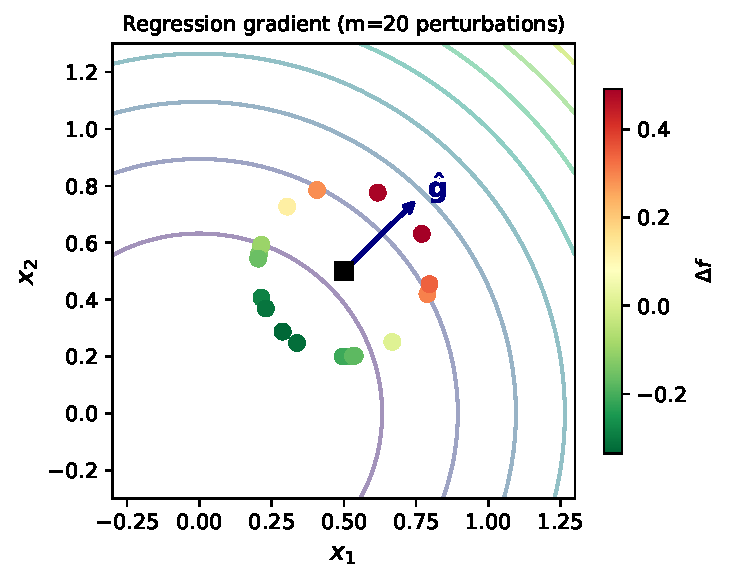
\includegraphics[width=0.95\linewidth]{fig_regression_gradient.pdf}\\
    {\scriptsize Sample perturbations colored by $\Delta f$ value.
     Navy arrow: estimated gradient direction.
     More perturbations yield a more accurate estimate.}

    \column{0.47\linewidth}
    \textbf{Reading the figure.}
    Each dot is one perturbation $\x + \Delta\x^{(i)}$, colored by
    whether $f$ increased (red) or decreased (green) relative to $f(\x)$.
    The regression fit finds the linear trend in these colors, and the
    direction of fastest increase is the estimated gradient (navy arrow).
    Points in the direction of the true gradient tend to be red;
    points in the opposite direction tend to be green.
  \end{columns}

  \medskip
  \textbf{Strengths:}
  \begin{itemize}
    \item Works for any black-box function, including non-differentiable
          or discontinuous functions (though the gradient estimate is then
          an approximation to a sub-gradient).
    \item Works even when $f$ is noisy (stochastic), because the
          least-squares fit averages out noise.
    \item Requires only $m + 1$ function evaluations
          (including $f(\x)$ itself).
  \end{itemize}

  \textbf{Limitations:}
  \begin{itemize}
    \item Requires $m \geq n$ evaluations to have an overdetermined system
          (more equations than unknowns), which becomes expensive for
          large $n$.
    \item Accuracy degrades in high dimensions --- with $m$ fixed, each
          individual direction is sampled less densely.
    \item For very large $n$, SPSA (next section) is far more efficient.
  \end{itemize}

  \begin{alertblock}{Key Takeaway}
    Regression gradient is a powerful tool for moderate-dimensional
    black-box optimization.  It bridges the gap between pure gradient
    methods (which need differentiable $f$) and derivative-free methods
    (which ignore gradient structure entirely).
  \end{alertblock}

\end{frame}

% =============================================================================
\section{6. SPSA}
% =============================================================================

\begin{frame}[allowframebreaks]{SPSA: Simultaneous Perturbation for Large-Scale Problems}

  The regression gradient requires at least $n+1$ function evaluations
  to estimate the gradient in $n$ dimensions.  For problems with hundreds
  of thousands of variables --- such as training a large neural network
  without automatic differentiation --- this is prohibitively expensive.

  \textbf{Simultaneous Perturbation Stochastic Approximation (SPSA)}
  estimates the gradient using only \textbf{2 function evaluations},
  regardless of the dimension $n$.  The price is noise: any single SPSA
  estimate has high variance, but the estimates are \emph{unbiased}
  (they are correct on average), so averaging over many iterations
  converges to the true gradient.

  \begin{block}{SPSA Core Idea}
    Instead of perturbing one coordinate at a time (as finite differences
    do), perturb \emph{all} coordinates simultaneously with a random
    $\pm 1$ vector $\mathbf{z}$.  The ratio
    $\dfrac{f(\x+\delta\mathbf{z}) - f(\x-\delta\mathbf{z})}{2\delta}$
    measures the directional derivative along $\mathbf{z}$.
    Multiplying by $z_i$ gives a noisy but unbiased estimate of
    $\partial f/\partial x_i$.
  \end{block}

  \begin{block}{SPSA Gradient Estimate (eq.\ 2.48)}
    Draw $\mathbf{z} \in \{-1,+1\}^n$ (a vector with each component
    independently $+1$ or $-1$ with equal probability).  Then:
    \[
      \hat{g}_i
      \;=\;
      \frac{f(\x + \delta\mathbf{z}) - f(\x - \delta\mathbf{z})}{2\delta}
      \cdot z_i
      \qquad\text{for each component }i
    \]
  \end{block}

  \begin{block}{Notation}
    \begin{itemize}
      \item $\delta$ (delta, a small positive number) is the perturbation
            radius: how far we move from $\x$ in the direction $\mathbf{z}$.
            Typical values: $\delta \in [0.01, 0.5]$ depending on the scale
            of $f$.
      \item $\mathbf{z} \in \{-1,+1\}^n$ is a Rademacher random vector:
            each component $z_i$ (``z sub i'') is independently $+1$ or $-1$
            with probability $1/2$ each.
      \item $\hat{g}_i$ (``g-hat sub i'') is the SPSA estimate of
            $\partial f / \partial x_i$.  The hat ($\hat{\phantom{x}}$)
            denotes an estimate rather than the true value.
    \end{itemize}
  \end{block}

  \framebreak

  \textbf{Why is $\hat{g}_i$ an unbiased estimator of $\partial f/\partial x_i$?}

  The central difference formula gives approximately:
  \[
    \frac{f(\x+\delta\mathbf{z}) - f(\x-\delta\mathbf{z})}{2\delta}
    \approx \nabla f(\x)^\top \mathbf{z}
    = \sum_{j=1}^{n} \frac{\partial f}{\partial x_j} z_j
  \]
  Multiplying by $z_i$ and taking expectation over $\mathbf{z}$:
  \[
    \mathbb{E}[\hat{g}_i]
    = \mathbb{E}\!\left[z_i \sum_{j=1}^n \frac{\partial f}{\partial x_j} z_j\right]
    = \sum_{j=1}^n \frac{\partial f}{\partial x_j} \mathbb{E}[z_i z_j]
    = \frac{\partial f}{\partial x_i}
  \]
  because $\mathbb{E}[z_i z_j] = 1$ if $i=j$ and $0$ otherwise
  (the components of $\mathbf{z}$ are independent).

  \medskip
  \textbf{Using multiple samples.}
  Average $m$ independent SPSA estimates to reduce variance:
  \[
    \hat{\mathbf{g}}
    = \frac{1}{m} \sum_{k=1}^{m} \hat{\mathbf{g}}^{(k)}
  \]
  where $\hat{\mathbf{g}}^{(k)}$ (``g-hat superscript $k$'') is the
  $k$-th estimate.  The variance decreases as $1/m$, so using $m=500$
  samples reduces variance by a factor of 500 at a cost of only $2m=1000$
  function evaluations.

\end{frame}

% ------------------------------------------------------------------------------
\begin{frame}[fragile]{SPSA: Python Implementation}
\begin{lstlisting}[caption={SPSA gradient estimation --- Python (NumPy)}]
import numpy as np

def spsa_gradient(f, x, delta=0.1, m=10):
    """
    SPSA gradient estimate using m pairs of perturbations.
    Total cost: 2*m function evaluations (independent of dimension n).
    For comparison, forward finite differences cost n+1 evaluations.
    """
    n = len(x)
    g = np.zeros(n)
    for _ in range(m):
        # Draw a Rademacher vector: each component is +1 or -1 uniformly
        z = np.random.choice([-1.0, 1.0], size=n)
        fp = f(x + delta * z)   # evaluate at x + delta*z
        fm = f(x - delta * z)   # evaluate at x - delta*z
        # Central difference along z, then multiply by z (component-wise)
        g += ((fp - fm) / (2 * delta)) * z
    return g / m    # average over m estimates

# Example: f(x, y) = x^2 + y^2 + 0.5*x*y
# True gradient at (1, 2): [2*1 + 0.5*2, 2*2 + 0.5*1] = [3.0, 4.5]
f = lambda x: x[0]**2 + x[1]**2 + 0.5*x[0]*x[1]
x0 = np.array([1.0, 2.0])
np.random.seed(0)
g_spsa = spsa_gradient(f, x0, delta=0.01, m=500)
print(f"SPSA estimate: {g_spsa}")   # approximately [3.0, 4.5]
print(f"True gradient: [3.0, 4.5]")
\end{lstlisting}
\end{frame}

% ------------------------------------------------------------------------------
\begin{frame}[allowframebreaks]{SPSA: Illustration and Comparison with Regression Gradient}

  \begin{columns}[T]
    \column{0.48\linewidth}
    \centering
    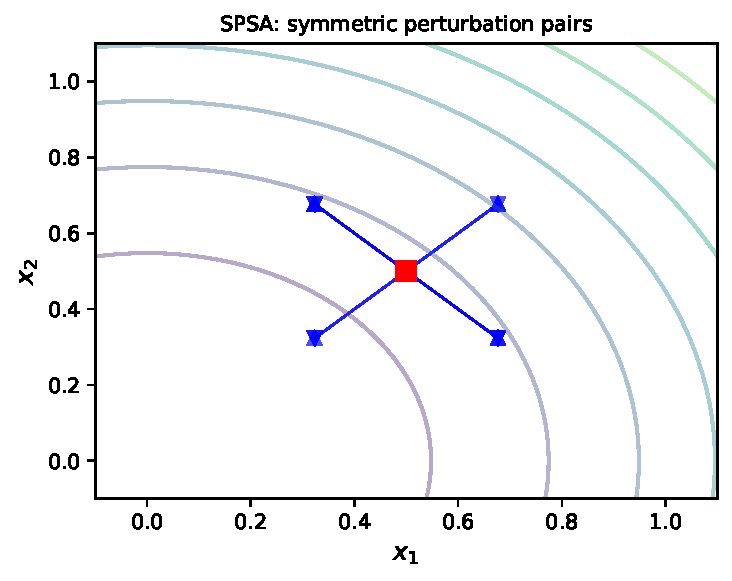
\includegraphics[width=0.95\linewidth]{fig_spsa.pdf}\\
    {\scriptsize Each SPSA iteration uses one symmetric pair of
    perturbations $\x\pm\delta\mathbf{z}$ (red and green dots).
    The estimated gradient direction (navy arrow) converges as
    more pairs are averaged.}

    \column{0.49\linewidth}
    \textbf{Reading the figure.}
    Each pair of colored dots represents one SPSA iteration: we step
    distance $\delta$ in the random direction $\mathbf{z}$ (green dot)
    and in the opposite direction (red dot).  The difference in $f$
    values divided by $2\delta$ gives a noisy slope, and multiplying
    by $\mathbf{z}$ distributes that slope to all $n$ gradient components.
    After averaging many pairs, the estimate converges to the true gradient.
  \end{columns}

  \medskip
  \begin{block}{SPSA vs.\ Regression Gradient: Summary Comparison}
    \renewcommand{\arraystretch}{1.4}
    \begin{tabular}{p{3cm}p{3.5cm}p{3.5cm}}
      \toprule
      \textbf{Property} & \textbf{Regression Gradient} & \textbf{SPSA} \\
      \midrule
      Evaluations per estimate & $m + 1$ & $2m$ \\
      Min.\ evaluations for 1 estimate & $n + 1$ (need $m \geq n$) & $2$ (any $m \geq 1$) \\
      Accuracy (fixed $m$) & Better (uses all directions) & Noisier (random) \\
      Scales to large $n$? & No ($m$ must grow with $n$) & Yes (always 2 per iter) \\
      Typical use case & Moderate $n$, noisy $f$ & Very large $n$, black-box \\
      \bottomrule
    \end{tabular}
  \end{block}

  \begin{alertblock}{Key Takeaway}
    SPSA is the preferred gradient estimator when $n$ is very large and
    $f$ is a black box.  Each individual estimate is noisy, but the
    estimates are unbiased, so gradient-descent-style optimization
    algorithms converge on average.  SPSA is widely used in reinforcement
    learning, neural architecture search, and the optimization of
    simulation-based systems.
  \end{alertblock}

\end{frame}

% =============================================================================
\section{7. Summary and Exercises}
% =============================================================================

\begin{frame}[allowframebreaks]{Chapter Summary: Core Concepts}

  This chapter has built up a complete toolkit for computing or estimating
  the derivative of a function.  We review the key ideas below.

  \begin{block}{Mathematical Objects}
    \begin{itemize}
      \item The \textbf{derivative} $f'(x)$ of a scalar function
            $f:\mathbb{R}\to\mathbb{R}$ measures the instantaneous rate of
            change of $f$ at $x$: it is the slope of the tangent line.
      \item The \textbf{gradient} $\nabla f(\x)$ (nabla f) of
            $f:\mathbb{R}^n\to\mathbb{R}$ is the vector of partial derivatives;
            it points in the direction of steepest ascent and has magnitude
            equal to the maximum rate of increase.
      \item The \textbf{Jacobian} $\mathbf{J}$ of a vector-valued function
            $\mathbf{f}:\mathbb{R}^n\to\mathbb{R}^m$ is the $m\times n$
            matrix of all partial derivatives; it generalizes the gradient to
            multi-output functions.
      \item The \textbf{Hessian} $\mathbf{H}$ is the $n\times n$ matrix of
            second-order partial derivatives; it captures the curvature of $f$
            and determines whether a critical point is a minimum, maximum, or
            saddle.
      \item The \textbf{directional derivative} $\nabla_\mathbf{s} f(\x)$
            measures the rate of change of $f$ in an arbitrary direction
            $\mathbf{s}$ and equals $\nabla f(\x)^\top \mathbf{s}$.
    \end{itemize}
  \end{block}

  \framebreak

  \begin{block}{Differentiation Methods (Ordered by Accuracy and Cost)}
    \begin{itemize}
      \item \textbf{Symbolic differentiation}: exact algebraic formula for
            $f'$; requires a closed-form expression for $f$; may suffer from
            expression swell.
      \item \textbf{Forward finite difference}: approximates $f'$ with $O(h)$
            error using 2 evaluations; simple but limited by step-size
            trade-offs.
      \item \textbf{Central finite difference}: $O(h^2)$ error, same 2
            evaluations; more accurate because even-order Taylor terms cancel.
      \item \textbf{Complex-step method}: near-machine-precision accuracy,
            no subtractive cancellation; requires complex arithmetic support.
      \item \textbf{Forward-mode AD}: exact derivatives using dual numbers;
            one pass per input; efficient for few inputs.
      \item \textbf{Reverse-mode AD (backpropagation)}: exact full gradient
            in one backward pass; $O(\text{graph})$ memory; ideal for scalar
            loss with many inputs (deep learning).
      \item \textbf{Regression gradient}: estimates gradient from
            $m+1$ black-box evaluations via least squares; works for noisy
            or non-differentiable $f$; cost grows with dimension.
      \item \textbf{SPSA}: unbiased gradient estimate from 2 evaluations
            regardless of dimension; noisier but scalable to very large $n$.
    \end{itemize}
  \end{block}

\end{frame}

% ------------------------------------------------------------------------------
\begin{frame}[allowframebreaks]{Summary: Textbook Section 2.7 Bullet Points Explained}

  The following points summarize the chapter's conclusions in the language
  of the textbook, with brief explanations.

  \medskip
  \textbf{1. Derivatives guide optimization.}
  Derivatives are useful in optimization because they provide information
  about how to change a given point to \emph{improve} the objective
  function.  Without this information, an optimizer must blindly probe
  the search space; with it, the optimizer can follow the gradient (or
  a Newton direction) to converge much faster.

  \medskip
  \textbf{2. Multivariate derivative objects.}
  For functions of multiple variables, the key derivative concepts are the
  \textbf{gradient} (first-order, direction of steepest change), the
  \textbf{Hessian} (second-order, curvature), and the
  \textbf{directional derivative} (rate of change along any chosen
  direction).  Together these direct the search for an optimum.

  \medskip
  \textbf{3. Finite difference approximations.}
  One approach to numerical differentiation is to replace the theoretical
  limit in the derivative definition with a small but finite step $h$.
  The three basic variants --- forward, central, and backward --- differ
  in their accuracy: central difference achieves $O(h^2)$ by exploiting
  symmetric cancellation of even-order error terms.

  \framebreak

  \textbf{4. The complex-step advantage.}
  The \textbf{complex-step method} can eliminate subtractive cancellation
  error entirely.  Because it extracts the imaginary part of a single
  complex evaluation rather than differencing two real evaluations, the
  step $h$ can be made arbitrarily small (e.g., $10^{-20}$) without any
  loss of precision.  The result is a near-machine-precision derivative
  estimate.

  \medskip
  \textbf{5. Automatic differentiation.}
  \textbf{Automatic differentiation} computes derivatives of a program
  by systematically applying the chain rule to each elementary operation
  in the computational graph.  Forward accumulation propagates tangents
  (one pass per input) using dual numbers; reverse accumulation
  (backpropagation) propagates adjoints (one pass for all inputs) by
  storing and replaying the computational tape.  Both give exact
  floating-point derivatives.

  \medskip
  \textbf{6. Regression gradient for black-box functions.}
  The \textbf{regression gradient} uses linear regression on a set of
  function evaluations at random perturbations to find the best-fit
  gradient vector.  It works for any function that can be evaluated,
  even black-box, noisy, or non-differentiable ones, and requires $m+1$
  evaluations.

  \medskip
  \textbf{7. SPSA for high-dimensional black-box problems.}
  \textbf{SPSA} allows unbiased gradient estimation for very high-dimensional
  functions using only 2 function evaluations per sample, regardless of
  dimension.  It is the method of choice when $n$ is huge and $f$ is a
  black box.

\end{frame}

% ------------------------------------------------------------------------------
\begin{frame}[allowframebreaks]{Selected Exercises with Full Solutions}

  \textbf{Exercise 2.1.}
  \emph{How can you approximate the Hessian matrix from the gradient using
  forward differences?}

  \begin{block}{Solution}
    The Hessian $\mathbf{H}$ has entries
    $H_{ij} = \partial^2 f / \partial x_i \partial x_j$.
    We can estimate the $j$-th column of $\mathbf{H}$ by applying
    forward difference to the gradient in the $j$-th direction:
    \[
      \mathbf{H}_{:,j}
      \approx
      \frac{\nabla f(\x + h\mathbf{e}_j) - \nabla f(\x)}{h}
    \]
    where $\mathbf{e}_j$ is the $j$-th standard basis vector.
    Repeating for each $j = 1, \ldots, n$ gives the full Hessian at
    cost $n+1$ gradient evaluations (each gradient costs $n$ evaluations
    if computed by finite differences, for a total of $O(n^2)$).
  \end{block}

  \medskip
  \textbf{Exercise 2.2.}
  \emph{What is a drawback of central differences compared with forward
  differences?}

  \begin{block}{Solution}
    Central difference requires \textbf{two function evaluations per
    dimension} --- one at $x + h/2$ and one at $x - h/2$ --- whereas
    forward difference requires only one extra evaluation (at $x+h$,
    since $f(x)$ is already known).  So for computing the gradient in $n$
    dimensions, central difference costs $2n$ evaluations vs.\ $n+1$ for
    forward difference.  This doubling of cost may matter when $f$ is
    expensive to evaluate.
  \end{block}

  \framebreak

  \textbf{Exercise 2.3.}
  \emph{Identify the dominant term in
  $f'(x) = \dfrac{1}{x} + e^x - \dfrac{1}{x^2}$ for small $x > 0$.}

  \begin{block}{Solution}
    For small $x$ (say $x = 0.1$):
    \begin{itemize}
      \item $e^x \approx 1 + x \approx 1$ (small, bounded)
      \item $1/x = 10$ (large)
      \item $1/x^2 = 100$ (very large, and negative in the expression)
    \end{itemize}
    The term $-1/x^2$ grows most rapidly as $x\to 0^+$, so
    $-1/x^2$ dominates.  The function approaches $-\infty$ as
    $x\to 0^+$.
  \end{block}

  \medskip
  \textbf{Exercise 2.4.}
  \emph{If $f(3 + ih) = 2 + 4ih$, what is $f'(3)$?}

  \begin{block}{Solution}
    By the complex-step formula:
    \[
      f'(3) \approx \frac{\operatorname{Im}(f(3+ih))}{h}
      = \frac{\operatorname{Im}(2 + 4ih)}{h}
      = \frac{4h}{h}
      = 4.
    \]
    So $f'(3) = 4$.  The real part gives $f(3) = 2$.
  \end{block}

  \framebreak

  \textbf{Exercise 2.6.}
  \emph{Combine forward and backward differences to estimate $f''(x)$.}

  \begin{block}{Solution}
    Observe that $f''(x)$ is the derivative of $f'(x)$.  We can apply
    finite difference to the derivative:
    \[
      f''(x)
      \approx \frac{f'(x + h/2) - f'(x - h/2)}{h}
    \]
    Now substitute the forward-difference approximation for each derivative:
    $f'(x+h/2) \approx [f(x+h) - f(x)]/h$ and
    $f'(x-h/2) \approx [f(x) - f(x-h)]/h$.
    Substituting:
    \[
      f''(x)
      \approx \frac{f(x+h) - 2f(x) + f(x-h)}{h^2}
    \]
    This requires three function evaluations: $f(x-h)$, $f(x)$, and
    $f(x+h)$.  The truncation error is $O(h^2)$.
  \end{block}

  \framebreak

  \textbf{Exercise 2.5.}
  \emph{Draw the computational graph for $f(x,y) = \sin(x + y^2)$
  and apply forward accumulation at $(x,y)=(1,1)$ to find
  $\partial f/\partial y$.}

  \begin{block}{Solution}
    The intermediate nodes are:
    $c_1 = y^2 = 1$;\quad
    $c_2 = x = 1$;\quad
    $c_3 = c_2 + c_1 = 2$;\quad
    $c_4 = \sin(c_3) = \sin(2)$.

    Seeding with $\dot{y}=1$, $\dot{x}=0$ and applying the chain rule
    at each node:
    \[
      \dot{c}_1 = 2y \cdot \dot{y} = 2\cdot 1 = 2; \qquad
      \dot{c}_2 = \dot{x} = 0; \qquad
      \dot{c}_3 = \dot{c}_2 + \dot{c}_1 = 0 + 2 = 2; \qquad
      \dot{c}_4 = \cos(c_3)\cdot\dot{c}_3 = \cos(2)\cdot 2.
    \]
    Therefore:
    \[
      \frac{\partial f}{\partial y}
      = \dot{c}_4
      = 2\cos(2)
      \approx 2\times(-0.4161)
      \approx -0.832.
    \]
    The negative sign tells us that increasing $y$ from $y=1$ while
    holding $x=1$ fixed decreases $f$.
  \end{block}

\end{frame}

% ------------------------------------------------------------------------------
\begin{frame}{Chapter 2: Concept Map}
  \centering
  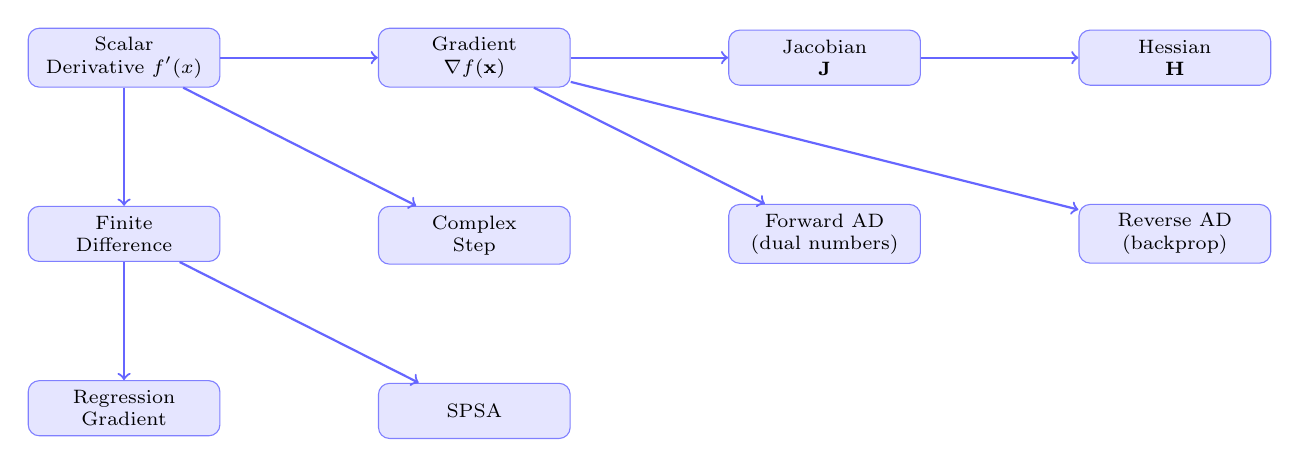
\begin{tikzpicture}[
    node distance=1.2cm and 2.0cm,
    box/.style={rectangle, rounded corners, draw=blue!50, fill=blue!10,
                text width=2.2cm, align=center, minimum height=0.7cm,
                font=\scriptsize},
    arrow/.style={->, thick, blue!60},
  ]
    \node[box] (deriv) {Scalar\\Derivative $f'(x)$};
    \node[box, right=of deriv] (grad)  {Gradient\\$\nabla f(\mathbf{x})$};
    \node[box, right=of grad]  (jac)   {Jacobian\\$\mathbf{J}$};
    \node[box, right=of jac]   (hess)  {Hessian\\$\mathbf{H}$};

    \node[box, below=1.5cm of deriv] (fd)   {Finite\\Difference};
    \node[box, below=1.5cm of grad]  (cplx) {Complex\\Step};
    \node[box, below=1.5cm of jac]   (fwd)  {Forward AD\\(dual numbers)};
    \node[box, below=1.5cm of hess]  (rev)  {Reverse AD\\(backprop)};

    \node[box, below=1.5cm of fd]    (rg)   {Regression\\Gradient};
    \node[box, below=1.5cm of cplx]  (spsa) {SPSA};

    \draw[arrow] (deriv) -- (grad);
    \draw[arrow] (grad)  -- (jac);
    \draw[arrow] (jac)   -- (hess);
    \draw[arrow] (deriv) -- (fd);
    \draw[arrow] (deriv) -- (cplx);
    \draw[arrow] (grad)  -- (fwd);
    \draw[arrow] (grad)  -- (rev);
    \draw[arrow] (fd)    -- (rg);
    \draw[arrow] (fd)    -- (spsa);
  \end{tikzpicture}
\end{frame}

% ------------------------------------------------------------------------------
\begin{frame}[allowframebreaks]{Method Selection Guide}

  To choose the right differentiation method for a given problem, consider
  the following decision criteria:

  \begin{block}{When to Use Which Method}
    \renewcommand{\arraystretch}{1.6}
    \begin{tabular}{p{3.5cm}p{3.2cm}p{4.5cm}}
      \toprule
      \textbf{Scenario} & \textbf{Recommended Method} & \textbf{Reason} \\
      \midrule
      $f$ has a closed algebraic formula
        & Symbolic differentiation
        & Exact; derivative is reusable \\
      Code-defined $f$, few inputs ($n$ small)
        & Forward-mode AD
        & One pass per input; exact \\
      Code-defined $f$, scalar output, many inputs
        & Reverse-mode AD
        & One backward pass for full gradient \\
      Black-box $f$, need high-accuracy gradient
        & Complex-step
        & Near-machine precision, no cancellation \\
      Black-box $f$, moderate $n$ ($n \lesssim 100$)
        & Regression gradient
        & Robust, overdetermined least squares \\
      Black-box $f$, very large $n$ ($n \gg 100$)
        & SPSA
        & Only 2 evaluations per estimate \\
      \bottomrule
    \end{tabular}
  \end{block}

  \begin{alertblock}{Practical Recommendation}
    For code written in NumPy or PyTorch, \textbf{automatic differentiation}
    (via JAX, PyTorch autograd, or similar) is almost always the best first
    choice: it is exact, efficient for both few-input and few-output
    functions, and requires no modification to your existing code
    (beyond using a JAX-compatible library).
    Reserve finite differences and SPSA for situations where AD is
    unavailable or impractical.
  \end{alertblock}

\end{frame}

% =============================================================================
\begin{frame}{References}
  \begin{thebibliography}{9}
    \bibitem{kochenderfer2026}
      M. J. Kochenderfer and T. A. Wheeler,
      \textit{Algorithms for Optimization}, 2nd ed.
      MIT Press, 2026.
    \bibitem{martins2003}
      J. R. R. A. Martins, P. Sturdza, and J. J. Alonso,
      ``The Complex-Step Derivative Approximation,''
      \textit{ACM Trans.\ Math.\ Softw.}, vol.\ 29, no.\ 3,
      pp.\ 245--262, 2003.
    \bibitem{baydin2018}
      A. G. Baydin et al.,
      ``Automatic Differentiation in Machine Learning: a Survey,''
      \textit{JMLR}, vol.\ 18, no.\ 153, 2018.
    \bibitem{spall1992}
      J. C. Spall,
      ``Multivariate Stochastic Approximation Using a Simultaneous
      Perturbation Gradient Approximation,''
      \textit{IEEE Trans.\ Autom.\ Control},
      vol.\ 37, no.\ 3, pp.\ 332--341, 1992.
  \end{thebibliography}
\end{frame}

\end{document}
